\documentclass[twoside,a4paper]{report}

\usepackage[bottom]{footmisc}
\usepackage[pdftex]{graphicx}
\usepackage{textcomp}
\usepackage[compact,nobottomtitles*]{titlesec}
\titleformat{\chapter}[display]
{\normalfont\bfseries}{}{0pt}{\huge}
\usepackage{lipsum}
\usepackage{wrapfig}
\usepackage{adjustbox}
\usepackage[utf8]{inputenc}
\usepackage[english,main=polish]{babel}
\usepackage[T1]{fontenc}
\usepackage[fit]{truncate}
\usepackage{array}
\usepackage{makecell}
\usepackage{float}
\usepackage{anysize}
\usepackage{enumitem}
\usepackage[font=small,labelfont=bf]{caption}
\usepackage{subcaption}
\usepackage{url}
\usepackage{hyperref}
\usepackage{csquotes}
\usepackage[
sorting=none
]{biblatex}
\emergencystretch=1em
\addbibresource{bibliografia.bib}
\usepackage{listings}
\renewcommand{\ttdefault}{pcr}
\usepackage{fancyhdr}
\usepackage{multirow}
\usepackage{tabularx}
\usepackage{indentfirst}
\usepackage{gensymb}
\raggedbottom

\newcolumntype{C}{>{\centering\arraybackslash}X}

\newcommand*{\noaddvspace}{\renewcommand*{\addvspace}[1]{}}
\addtocontents{lof}{\protect\noaddvspace}

\pagestyle{fancy}
\fancyhf{}

\renewcommand{\lstlistlistingname}{Spis listingów}

\lstdefinelanguage{JavaScript}{
    keywords={function, class, extends, return, render},
}

\lstdefinelanguage{Elm}{
    keywords={type, alias, update, case, of, init, view, subscriptions, let, in, viewDate, viewTime},
}

\lstset{
  basicstyle=\ttfamily,
  keywordstyle=\textbf,
  columns=fullflexible,
  frame=single,
  breaklines=true,
}

\renewcommand{\chaptermark}[1]{\markboth{#1}{}}
\renewcommand{\sectionmark}[1]{\markright{\thesection\ #1}}
\renewcommand{\headrulewidth}{0.5pt}
\renewcommand{\footrulewidth}{0pt}

\fancyhead[LE,RO]{\bfseries\thepage}
\fancyhead[LO]{\nouppercase{\bfseries{\truncate{.95\headwidth}{\rightmark}}}}
\fancyhead[RE]{\nouppercase{\bfseries{\truncate{.95\headwidth}{\leftmark}}}}

\titlespacing*{\chapter}{0pt}{-50pt}{20pt}

\linespread{1.5}

\parskip0.05in

\marginsize{3.5cm}{2.5cm}{2.5cm}{2.5cm}
\fancyhfoffset[E,O]{0pt}

% ---------------------------------------------------------------------------------------------------------------------

\begin{document}

% allows useg @ as a @ not as special character
% required for macro redefinition
\makeatletter

% parameters definition
% they cannot conflict with other
% like bibteh attributes etc.
\def\tytul#1{\def\@tytul{#1}}
\def\promotor#1{\def\@promotor{#1}}
\def\miasto#1{\def\@miasto{#1}}
\def\studies#1{\def\@studies{#1}}
\def\descr#1{\def\@descr{#1}}
\def\indeks#1{\def\@indeks{#1}}
\def\dept#1{\def\@dept{#1}}
\def\spec#1{\def\@spec{#1}}

\def\maketitle{
    %removal of header
    \keepXColumns
    \thispagestyle{empty}%
    \begin{center}
        \begin{tabularx}{\textwidth}{CcC}
            \multirow{4}{*}{
\includegraphics[height=2.35cm]{img/logo_pg.png}}
          & \textsc{\textbf{Politechnika Gdańska}} &
          \multirow{4}{*}{
\includegraphics[height=2.35cm]{img/logo_eti.png}}
       \\ & & \\
          & \textsc{\textbf{Wydział Elektroniki, }}& \\
          & \textsc{\textbf{Telekomunikacji i Informatyki }}& \\
        \end{tabularx}
    \end{center}
    \begin{center}
        \begin{tabularx}{\textwidth}{XX}
            \textbf{Katedra:} & \@dept\\
                              &\\
            \textbf{Imię i nazwisko dyplomanta:} & \@author\\
                                                 &\\
            \textbf{Nr albumu:} & \@indeks\\
                                &\\
            \textbf{Forma i poziom studiów:} & \@studies\\
                                             &\\
            \textbf{Kierunek studiów:} & Informatyka\\
                                       &\\
            \textbf{Specjalność:} & \@spec
        \end{tabularx}
    \end{center}
    \begin{center}
        \Large{\textbf{Praca dyplomowa magisterska}}
    \end{center}
    \vspace{1cm}
    \begin{tabular}{l}
        \textbf{Temat pracy:} \\ \@tytul\\
        \\
        \textbf{Title of thesis:} \\ \@title\\
        \\
        \textbf{Opiekun pracy:} \\ \@promotor\\
        \\
        \textbf{Data ostatecznego zatwierdzenia raportu podobieństw w JSA:} TBA
    \end{tabular}
    \vspace*{\stretch{6}}
    \begin{center}
        \@miasto, \@date
    \end{center}

}

%restore @ sign
\makeatother

\cleardoublepage


\tytul{Wykorzystanie języka Elm do tworzenia aplikacji frontendowych.}
\title{Programming the front-end applications with Elm language.}
\author{Marcin Jurczak}
\date{2022}
\miasto{Gdańsk}
\promotor{dr\ inż.\ Krzysztof Manuszewski}
\studies{Stacjonarne jednolite studia magisterskie}
\indeks{171641}
\dept{Algorytmów i Modelowania Systemów}
\spec{Algorytmów i Technologii Internetowych}

\maketitle
\clearpage
\pagenumbering{arabic}

% ---------------------------------------------------------------------------------------------------------------------

\chapter*{Streszczenie}
\noindent
Celem niniejszej pracy magisterskiej było stworzenie frontend'owej aplikacji internetowej z wykorzystaniem funkcyjnego języka Elm, porównanie tejże technologii z istniejącymi, bardziej powszechnymi rozwiązaniami tego typu, a także przygotowanie instrukcji laboratoryjnej, która mogłaby zostać wykorzystana w ramach zajęć \textit{,,Współczesne Aplikacje Programowania Funkcyjnego''} przeprowadzanych na Wydziale Elektroniki, Telekomunikacji i Informatyki Politechniki Gdańskiej.
Wytworzona aplikacja to strona internetowa typu \textit{startpage}, czyli startowa strona przeglądarki, zawierająca najpotrzebniejsze informacje, takie jak czas, pogoda oraz odnośniki do wyszukiwarki i najczęściej odwiedzanych stron.

\textbf{Słowa kluczowe:} Elm, programowanie funkcyjne, wytwarzane aplikacji internetowych

\textbf{Dziedzina nauki i techniki: }Nauki inżynieryjne i techniczne, inżynieria informatyczna.

\vspace{80pt}
{\let\clearpage\relax\chapter*{Abstract}}
\noindent
The goal of this master thesis is to use the Elm language to create a frontend web application, comparing this technology to existing, more popular solutions, as well as preparing a lab instruction, which could be used at \textit{,,Modern applications of functional programming''} class at Gdańsk University of Technology’s Faculty of Electronics, Telecommunications and Informatics.
The created application is a \textit{startpage}, meaning a starting page of a web browser consisting of the most useful information, such as time, weather and references to search engine and the most visited websites.

\textbf{Keywords:} Elm, functional programming, web development

\textbf{Field of Science and Technology:} Engineering and Technology, Information engineering.

% ---------------------------------------------------------------------------------------------------------------------

\tableofcontents

% ---------------------------------------------------------------------------------------------------------------------

\chapter*{Wykaz najważniejszych skrótów}
\begin{tabular}{rcl}
    \textbf{API} &---& ang.~Application Programming Interface,\\
                 &   & pol.~interfejs programowania aplikacji\\
    \textbf{CD} &---& ang.~Continuous Delivery, pol.~ciągłe dostarczanie\\
    \textbf{CI} &---& ang.~Continuous Integration, pol.~ciągła integracja\\
    \textbf{CSS} &---& ang.~Cascading Style Sheets, pol.~kaskadowe arkusze stylów\\
    \textbf{HTML} &---& ang.~Hypertext Markup Language, pol.~hipertekstowy język znaczników\\
    \textbf{HTTP} &---& ang.~Hypertext Transfer Protocol, pol.~protokół przesyłania hipertekstu\\
    \textbf{JSON} &---& ang.~JavaScript Object Notation, pol.~tekstowy format zapisu danych\\
    \textbf{SPA} &---& ang.~Single Page Application, pol.~jednostronicowa aplikacja internetowa\\
    \textbf{DOM} &---& ang.~Document Object Model, pol.~obiektowy model dokumentu\\
\end{tabular}

% ---------------------------------------------------------------------------------------------------------------------

\chapter{Wstęp i cel pracy}
\begin{wrapfigure}{r}{0.28\textwidth}
    \centering
    
\includegraphics[width=0.28\textwidth]{img/elm_logo.png}
    \caption*{Logo Elma}\label{fig:elm_logo}
\end{wrapfigure}

Głównym celem niniejszej pracy jest zapoznanie się z funkcyjnym językiem programowania Elm oraz stworzenie przykładowej frontendowej aplikacji internetowej.
Ponadto chciałbym przeprowadzić porównanie tej technologii z innymi, bardziej powszechnie używanymi rozwiązaniami do tworzenia aplikacji internetowych.
Ostatnim celem pracy jest przygotowanie części dydaktycznej w postaci instrukcji laboratoryjnej, która przeprowadza czytelnika przez cały proces tworzenia oprogramowania w języku Elm, od przygotowania środowiska, przed podstawy języka, po stworzenie aplikacji frontendowej.
Stworzona instrukcja mogłaby zostać potencjalnie wykorzystana w ramach przedmiotu Współczesne Aplikacje Programowania Funkcyjnego, prowadzonego przez mojego promotora, dra inż. Krzysztofa Manuszewskiego.

W drugim rozdziale skupiam się na przedstawieniu technologii powszechnie używanych do tworzenia frontendowych aplikacji internetowych, t.j. React.js, Angular oraz Vue.js.
Przedstawiam ich cechy charakterystyczne oraz proste przykłady tworzenia oprogramowania z ich użyciem.
Ponadto opisuję podobieństwa i różnice między nimi.

Trzeci rozdział poświęcam na wysokopoziomowe wprowadzenie do języka Elm.
Mówię o idei jaka przyświecała autorowi podczas tworzenia tego języka, jakie są jego potencjalne zastosowania i gdzie sprawdza się najlepiej.
Wprowadzam koncept \textit{The Elm Architecture} a także przedstawiam narzędzia wspomagające tworzenie oprogramowania z użyciem tejże technologii, włączając w to dokumentację.

W czwartym rozdziale przedstawiam implementację przygotowanej aplikacji frontendowej napisanej w Elmie.
Jest to poniekąd rozwinięcie poprzedniego rozdziału, ponieważ głównym celem jest dalej zapoznanie się z Elmem, jednak tutaj uwagę skupiam na przedstawieniu konkretnych rozwiązań technicznych, jakie zostały wykorzystane do osiągnięcia wybranego celu.

Piąty rozdział zawiera instrukcję laboratoryjną, w której przeprowadzam czytelnika nieposiadającego żadnego doświadczenia z Elmem przez proces tworzenia oprogramowania z wykorzystaniem tej technologii, zaczynając od przygotowania środowiska deweloperskiego, przez zupełne podstawy języka, aż po stworzenie aplikacji frontendowej przedstawionej we wcześniejszym rozdziale.

Szósty rozdział poświęcam na omówienie zagadnień związanych z ciągłą integracją oraz ciągłym dostarczaniem, a także przedstawiam narzędzia wykorzystywane przeze mnie w tym celu podczas tworzenia omawianej aplikacji.
Pokazuję, że Elm nie stanowi przeszkody w wykorzystywaniu tych technologii i całkowicie nadaje się do użytku produkcyjnego.

Ostatni rozdział dotyczy przede wszystkim podsumowania niniejszej pracy magisterskiej.
Przedstawiam produkt dwóch semestrów moich działań oraz wyciągam wnioski na temat Elma jako języka przeznaczonego do tworzenia aplikacji frontendowych.

Na końcu dokumentu znajdują się spisy użytych rysunków i listingów, a także bibliografia, która została wykorzystana podczas pracy nad niniejszym dokumentem oraz w czasie zapoznawania się z tematem wytwarzania aplikacji internetowych z wykorzystaniem języka Elm.

% ---------------------------------------------------------------------------------------------------------------------

\chapter{Powszechne rozwiązania}
W poniższym rozdziale chciałbym przedstawić najpopularniejsze rozwiązania do tworzenia frontendowych stron internetowych, które są powszechnie stosowane zarówno przez największych gigantów technologicznych, tj. Google, Facebook, Netflix, ale także małe, dopiero wchodzące na rynek firmy startupowe.

Według ankiety przeprowadzonej w 2021 roku przez StackOverflow~\cite{stacksurvey}, najczęściej wybieranym przez programistów rozwiązaniem do tworzenia stron internetowych była biblioteka React.js (40,14\% odpowiedzi), a na czwartym i piątym miejscu znajdowały się odpowiednio frameworki Angular (22,96\% odpowiedzi) oraz Vue.js (18,97\% odpowiedzi).

Ze względu na popularność wspomnianych rozwiązań, są to biblioteki i frameworki, na których chciałbym się skupić w poniższych podrozdziałach.
Opiszę, czym się charakteryzują, jakie są ich wady i zalety, a także co je ze sobą łączy oraz w jaki sposób są od siebie różne.

\section{React.js}
\begin{wrapfigure}{r}{0.2\textwidth}
    \centering
    
\includegraphics[width=0.2\textwidth]{img/logo_react.png}
    \caption*{Logo Reacta}\label{fig:logo_react}
\end{wrapfigure}
React.js~\cite{react} jest otwartoźródłową biblioteką języka programowania JavaScript, której głównym przeznaczeniem jest tworzenie interfejsów graficznych aplikacji internetowych, w większości wykorzystywana jest do aplikacji typu SPA\@.

Została stworzona w 2013 roku przez ówczesnego programistę Facebook'a, Jordana Walke.
Rozwój Reacta utrzymywany jest po dzień dzisiejszy przez~,,matczyną'' firmę Meta (dawniej znaną jako Facebook), a także przez społeczność indywidualnych programistów i innych organizacji ze względu na swoją otwartoźródłową naturę.

Tworzenie oprogramowania z użyciem tej biblioteki odbywa się poprzez budowanie nowych komponentów, które za pośrednictwem metody \texttt{render()} decydują, co ma zostać wyświetlane na ekranie użytkownika.
Odnosząc się do dokumentacji Reacta~\cite{reactdocs}, komponenty mogą być zdefiniowane na dwa sposoby: poprzez stworzenie JavaScript'owej funkcji lub wykorzystując klasę bazującą na \texttt{React.Component}.

Przykłady wspomnianych definicji zostały przedstawione odpowiednio na listingach~\ref{lst:func_comp} oraz~\ref{lst:class_comp}, a ich funkcjonalność jest jednakowa --- wyświetlenie napisu w formie nagłówka tagu \texttt{<h1>} o treści~,,\textit{Hello, }'' + imię zawarte w zmiennej \texttt{props}.

\begin{lstlisting}[caption={Funkcyjny komponent},label={lst:func_comp},language=JavaScript]
function Hello(props) {
  return <h1>Hello, {props.name}</h1>;
}
\end{lstlisting}
\begin{lstlisting}[caption={Klasowy komponent},label={lst:class_comp},language=JavaScript]
class Hello extends React.Component {
  render() {
    return <h1>Hello, {this.props.name}</h1>;
  }
}
\end{lstlisting}

Jedną z cech kodu tworzonego z użyciem biblioteki React jest jego deklaratywność.
Aby użyć stworzonego komponentu wystarczy go zaimportować i wykorzystać za pomocą tagu, dla powyższego przykładu tagu \texttt{<Hello name="Marcin"/>}, który dodatkowo zawiera pojedynczy argument \texttt{props}, będący obiektem z danymi, w tym przypadku zawierający imię~,,Marcin''.
Dzięki temu kod pisany przy pomocy biblioteki React jest bardzo reużywalny i pozwala na wykorzystanie komponentów nawet pomiędzy odrębnymi aplikacjami.

Jedną z zalet tego rozwiązania jest jego niesamowita popularność oraz dostępność gotowych rozwiązań.
W Internecie znajduje się mnóstwo poradników i instrukcji pomagających nowym użytkownikom zapoznać się z biblioteką i stworzyć pierwsze proste projekty.
Istnieje także dostatek pomocy dla bardziej zaawansowanych programistów Reacta oraz szeroka społeczność użytkowników chętnych do pomocy przy rozwiązywaniu bardziej skomplikowanych problemów.
Dostępność gotowych rozwiązań pozwala na relatywnie łatwy rozwój oprogramowania poprzez ich wykorzystanie.

Warto także wspomnieć, że React jest jedynie biblioteką, a nie pełnoprawnym frameworkiem.
Daje to programiście większą kontrolę nad tworzonym oprogramowaniem, ale także wymaga od niego większej odpowiedzialności w organizacji i utrzymaniu architektury aplikacji.

Istnieją także różne zestawy narzędzi do Reacta, które pozwalają na łatwiejsze tworzenie aplikacji z użyciem tej biblioteki, w zależności od potrzeb.
\textit{Create React App} pozwala na szybkie stworzenie prostej aplikacji jednostronicowej i zapewnia dogodne środowisko do nauki Reacta.
Do stworzenia strony internetowej renderowanej po stronie serwera z użyciem Node.js można skorzystać z \textit{Next.js}.
Natomiast do tworzenia statycznych stron internetowych przydatny może się okazać framework \textit{Gatsby}.
Istnieją także bardziej elastyczne zestawy narzędziowe oferujące większą dowolność konfiguracji, czego przykładami mogą być \textit{Neutrino}, \textit{Nx}, \textit{Parcel} czy \textit{Razzle}.

\section{Angular}
\begin{wrapfigure}{r}{0.2\textwidth}
    \centering
    
\includegraphics[width=0.2\textwidth]{img/logo_angular.png}
    \caption*{Logo Angulara}\label{fig:logo_angular}
\end{wrapfigure}
Angular~\cite{angulardocs} został stworzony przez firmę Google w 2016 roku z wykorzystaniem języka TypeScript --- nadzbioru języka JavaScript, który dodatkowo udostępnia takie funkcjonalności jak statyczne typowanie czy programowanie zorientowane obiektowo.
Pojęcie~,,nadzbioru'' oznacza w tym przypadku, że każdy program napisany w JavaScript jest także prawidłowym programem TypeScript.
Angular początkowo miał być drugą wersją biblioteki AngularJS, jednak w ostateczności Google zdecydował się wydać tę bibliotekę jako osobny produkt.

Angular, w przeciwieństwie do biblioteki React, jest pełnoprawnym \textit{frameworkiem}.
Biblioteka jest jedynie zbiorem funkcji i klas, które odpowiadają za konkretne zagadnienie i programista używa ich w celu rozwiązania określonego problemu.
Krótko mówiąc, to programista ma kontrolę nad wykonywanym kodem.

Framework często określa się jako~,,szkielet'' programu.
Udostępnia programiście gotowe środowisko do tworzenia aplikacji, dzięki czemu nie musi się martwić takimi procesami jak obsługiwanie żądań, różnych adresów URL, czy zajmowanie się ciasteczkami.
Wszystkie te rzeczy robi za programistę framework.
Znacznie ułatwia to proces tworzenia aplikacji, gdyż umożliwia uniknąć programowania powtarzalnych rzeczy wymaganych do prawidłowego działania aplikacji, a pozwala programiście skupić się na wdrażaniu logiki biznesowej.
Oznacza to także, że framework sprawuje większą kontrolę nad aplikacją niż programista, który~,,dowodzi'' jedynie chwilowo, po czym kontrola wraca do frameworka.

Głównym przeznaczeniem Angulara, podobnie jak w przypadku React.js, jest tworzenie aplikacji typu SPA\@.
Kolejnym podobieństwem jest jego deklaratywność, modularność i zorientowanie na komponenty, które mogą być reużywalne pomiędzy różnymi projektami.

Do stowrzenia nowego środowiska i projektu bardzo pomocne jest wykorzystanie narzędzia CLI od Angulara --- \texttt{ng}.
Komenda \texttt{ng new hello-world} pobierze wymagane dependencje przy użyciu menadżera paczek \texttt{npm}, utworzy nowe środowisko o wybranej nazwie (tutaj \textit{hello-world}), stworzy szkielet aplikacji w podfolderze \texttt{src/app}, a także doda odpowiednie plki konfiguracyjne.

Program jest od razu gotowy do uruchomienia w lokalnym środowisku przy pomocy polecenia \texttt{ng serve --open}.
Jest to prosta aplikacja powitalna, zawierająca jeden komponent \texttt{AppComponent}.
Kolejne komponenty mogą być dodawane z użyciem polecenia \texttt{ng generate component xyz}.
Na listingu~\ref{lst:angular_comp} został przedstawiony domyślny komponent w Angularze utworzony przy pomocy wspomnianego narzędzia.

\begin{lstlisting}[caption={Domyślny komponent w Angularze},label={lst:angular_comp},language=JavaScript]
@Component({
  selector: 'app-root',
  templateUrl: './app.component.html',
  styleUrls: ['./app.component.css']
})
export class AppComponent {
  title = 'hello-world';
}
\end{lstlisting}

Komponent, podobnie jak w przypadku Reacta, może zostać deklaratywnie wywołany w głównym pliku \texttt{main.ts} za pomocą zdefiniowanego selektora (tutaj \texttt{app-root}).
W trakcie generowania kodu zostają także dodane szablonowe pliki HTML oraz arkusze stylów CSS\@.

\section{Vue.js}
\begin{wrapfigure}{r}{0.2\textwidth}
    \centering
    
\includegraphics[width=0.2\textwidth]{img/logo_vue.png}
    \caption*{Logo Vue}\label{fig:logo_vue}
\end{wrapfigure}
Vue.js~\cite{vuejsdocs} jest otwortoźródłowym frameworkiem JavaScript, którego celem jest, podobnie jak w poprzednich przykładach, tworzenie interfejsów użytkownika w aplikacjach internetowych.

Wykorzystuje wirtualny DOM pozwalający na szybsze renderowanie stron.
Dzieje się to dzięki wirtualnej reprezentacji drzewa DOM jako obiekt JavaScriptowy, gdzie po każdej naniesionej zmianie tworzony jest nowy obiekt, a następnie są one między sobą porównywane i na koniec faktyczny DOM jest aktualizowany, co pozwala na znacznie przyspieszenie procesu renderowania strony, w porównaniu do każdorazowego nadpisywania drzewa DOM\@.

\section{Podobieństwa i różnice}

// TODO porównać frameworki

% ---------------------------------------------------------------------------------------------------------------------

\chapter{Elm}
Elm~\cite{elmdocs} jest czysto funkcyjnym językiem programowania przeznaczonym do tworzenia graficznych interfejsów użytkownika.
Powstał w roku 2012 wraz z opublikowaniem przez Evana Czaplickiego pracy~,,Elm: Concurrent FRP for Functional GUIs''~\cite{Czaplicki2012ElmC}.
Podczas jego tworzenia nacisk został położony na użyteczność, wydajność oraz niską podatność na błędy.

Składnia Elma jest mocno zbliżona do Haskella, a sam język jest kompilowany do JavaScriptu.
Wykorzystuje wirtualny DOM, czyli wirtualną reprezentację~,,prawdziwego'' drzewa DOM w postaci obiektu JavScriptowegoco pozwala na znacznie szybsze renderowanie stron internetowych w porównaniu do~,,regularnego'' DOM\@.

Największym atutem tego języka jest zdecydowanie silnie promowany przez autora brak występowania wyjątków w czasie działania programu (tzw. \textit{runtime exception}), co jest możliwe dzięki statycznemu sprawdzaniu typów przez kompilator Elma.

Celem kolejnych sekcji jest pokazanie na prostym przykładzie czym jest \textit{The Elm Architecture}, a także przedstawienie i opisanie narzędzi dostępnych podczas pracy z językiem Elm, zarówno tych dostarczanych domyślnie z platformą jak i tych od niezależnych twórców.

\section{The Elm Architecture}
\begin{figure}[H]
    \centering
    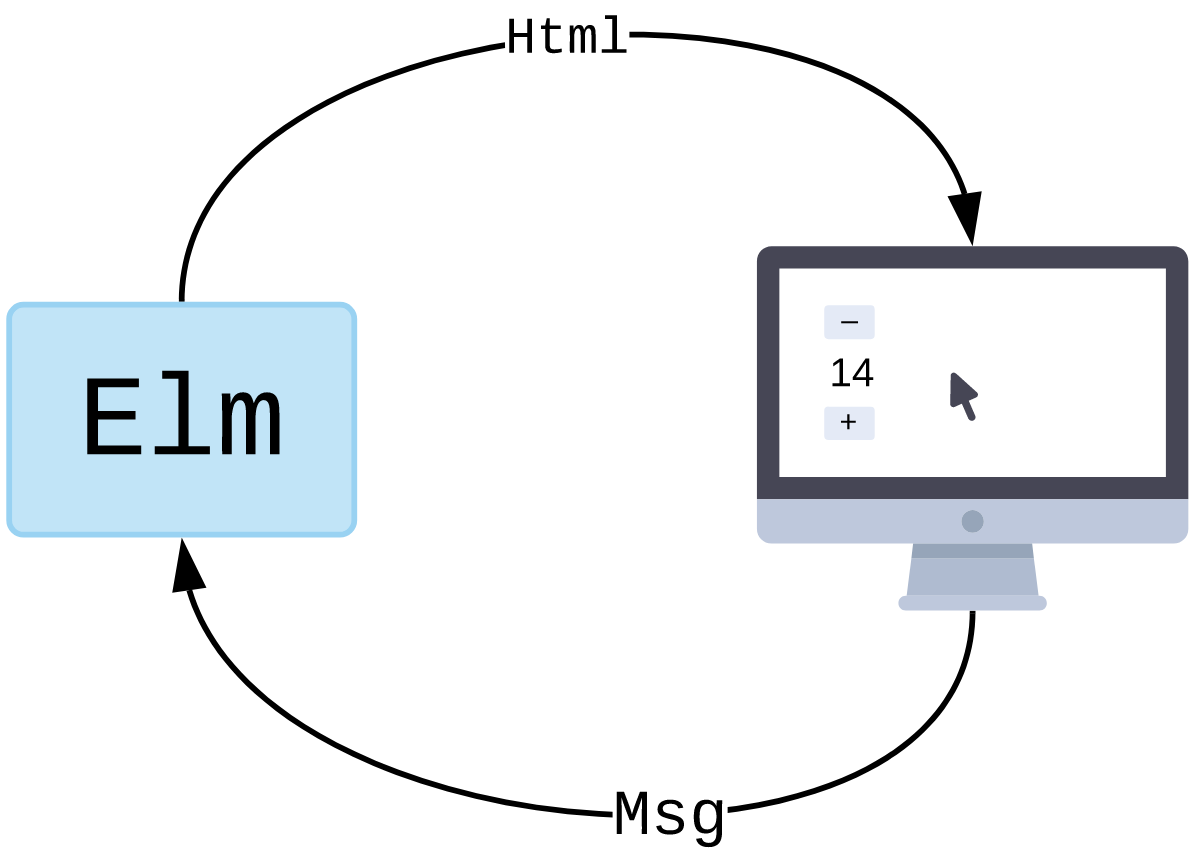
\includegraphics[width=0.5\textwidth]{img/elm_arch.png}
    \caption{Diagram działania programu w Elmie}\label{fig:elm_arch}
\end{figure}

\textit{The Elm Architecture} jest schematem tworzenia interaktywnych aplikacji internetowych lub gier.
Zgodnie z rysunkiem~\ref{fig:elm_arch} typowa aplikacja Elm działa w następujący sposób:
Program generuje pewien kod HTML, który zostaje wyświetlony na ekranie, a następnie komputer zwraca wiadomości informujące o tym co się dzieje, np.~użytkownik wcisnął guzik.

A co się dzieje wewnątrz wspomnianego programu Elmowego? Zawsze składa się z trzech podstawowych elementów:
\begin{itemize}[noitemsep,topsep=0pt]
    \item Model --- opisujący stan aplikacji
    \item Update --- opisujący logikę aplikacji
    \item View --- opisujący wygląd aplikacji
\end{itemize}

W kolejnych podrozdziałach przedstawiam powyższe elementy architektury Elma na podstawie prostego programu, którego zadaniem jest wyświetlenie na ekranie dwóch guzików oraz licznika, który może się zwiększać i zmniejszać, w zależności od tego, który guzik zostanie naciśnięty przez użytkownika.

\subsection{Model}
\begin{minipage}{.50\textwidth}
    Celem modelu przedstawionego na listingu~\ref{lst:Model} jest zdefiniowanie danych w naszej aplikacji.

    W tym przypadku model będzie bardzo prosty --- jest to rekord zawierający jedną wartość całkowitoliczbową (typ \texttt{Int}), która będzie mogła zostać zwiększona lub zmniejszona poprzez naciśnięcie odpowiedniego guzika.
\end{minipage}\hfill
\begin{minipage}{.43\textwidth}
\begin{lstlisting}[caption={\textit{The Elm Architecture} --- Model},label={lst:Model},language={Elm}]
type alias Model = Int

init : Model
init =
  0
    \end{lstlisting}
\end{minipage}\hfill

\subsection{Update}
\begin{minipage}{.43\textwidth}
    \begin{lstlisting}[caption={\textit{The Elm Architecture} --- Update},label={lst:Update},language={Elm}]
type Msg
  = Increment
  | Decrement

update : Msg -> Model -> Model
update msg model =
  case msg of
    Increment ->
      model + 1

    Decrement ->
      model - 1
    \end{lstlisting}
\end{minipage}\hfill
\begin{minipage}{.50\textwidth}
    Funkcja \texttt{update}, która została przedstawiona na listingu~\ref{lst:Update}, ma za zadanie opisywać jak nasz model będzie się zmieniał w czasie.

    Jako argument przyjmuje nowo zdefiniowany typ \texttt{Msg}, który ma dwa warianty --- \texttt{Increment} i \texttt{Decrement}. Typ zostaje dopasowany i w zależności od otrzymanego wariantu, model zostanie odpowiednio zaktualizowany (zmniejszony lub zwiększony) i zwrócony z funkcji.
\end{minipage}\hfill

\subsection{View}
Funkcja \texttt{view}, która została zaprezentowana na listingu~\ref{lst:View}, jako argument przyjmuje model i zwraca kod HTML\@.
Wykorzystany został tutaj handler \texttt{onClick} z biblioteki \texttt{Html.Events}, który po kliknięciu guzika, do którego został przypisany, generuje odpowiednią wiadomość.
Znak plusa generuje wiadomość \texttt{Increment}, znak minusa \texttt{Decrement}.
Następnie wybrana wiadomość trafia do funkcji \texttt{update}.

\begin{lstlisting}[caption={\textit{The Elm Architecture} --- View},label={lst:View},language={Elm}]
view : Model -> Html Msg
view model =
  div []
    [ button [ onClick Decrement ] [ text "-" ]
    , div [] [ text (String.fromInt model) ]
    , button [ onClick Increment ] [ text "+" ]
    ]
\end{lstlisting}

\section{Narzędzia}
Platforma Elm jest dostarczana wraz z zestawem narzędzi pozwalających m.in.~na kompilację plików źródłowych czy instalację dodatkowych modułów. Poniżej postaram się opisać większość z tych narzędzi, tj.~dostarczanych przez Elma, ale wskazać również te dostarczane przez zewnętrznych twórców, a które znacząco ułatwiły mi pracę z tym językiem.
\begin{center}
    \begin{tabularx}{\textwidth}{clX}
        \texttt{elm repl} &---& otwiera interaktywną sesję programistyczną.\\
        \texttt{elm init} &---& inicjalizuje bieżący katalog jako nowy projekt Elma poprzez stworzenie pliku \texttt{elm.json} opisującego projekt i jego zależności, a także tworzy katalog \texttt{src/}, w którym będą znajdowały się pliki \texttt{.elm}.\\
        \texttt{elm reactor} &---& uruchamia serwer deweloperski, który poprzez przeglądarkę pozwala wybrać dany plik źródłowy, skompilować go i sprawdzić jak wygląda po zbudowaniu.\\
        \texttt{elm make} &---& pozwala na kompilację kodu źródłowego do HTML'a lub JavaScript'u. Jest to najbardziej ogólna forma kompilacji, jaką udostępnia Elm, ale jest to niezwykle przydatne narzędzie, kiedy projekt stanie się zbyt skomplikowany na korzystanie z \texttt{elm reactor.}\\
        \texttt{elm install} &---& pozwala instalować paczki dostępne na stronie \url{package.elm-lang.org}, które udostępniają nowe funkcjonalności, jak np.~obsługa plików JSON czy praca z zapytaniami HTTP.\\
        \makecell{\texttt{elm-format}~\cite{elm-format}} &---& formater kodu~,,upiększający'' kod źródłowy Elm'a zgodnie z oficjalną dokumentacją opisującą styl jego tworzenia\\
        \makecell{\texttt{elm-live}~\cite{elm-live}} &---& podobnie jak \texttt{elm reactor}, uruchamia serwer deweloperski, jednak jest to znacznie bardziej rozbudowane narzędzie, oferujące m.in.~takie funkcjonalności jak kompilowanie Elm'a do JavaScript'u, załączanie go do pliku HTML i wyświetlanie w przeglądarce stworzonej strony\\
    \end{tabularx}
\end{center}

Ponadto, Elm posiada szeroką dokumentację, która w znacznym zakresie została wykorzystana podczas pracy nad niniejszym dokumentem.
Składa się z dwóch głównych części --- oficjalnego poradnika języka oraz technicznego opisu paczek, zarówno tych podstawowych jak i tych stworzonych i udostępnionych przez użytkowników.

Pierwsza część składa się z poradnika, który opisuje m.in.~podstawowe mechanizmy języka, przedstawia przykłady prostych aplikacji wraz z ćwiczeniami pozwalających na rozwijanie swojej znajomości Elma oraz umiejętności tworzenia oprogramowania z jego wykorzystaniem, a także oferuje wskazówki odnośnie dobrych praktyk pisania kodu w tym języku.

Druga część dokumentacji zawiera techniczny opis zarówno tych fundamentalnych modułów języka, niezbędnych do tworzenia aplikacji internetowych, takich jak \texttt{elm/core} i \texttt{elm/browser}, przez te mniej niezbędne, jednakowoż w wielu przypadkach wymagane do spełnienia podstawowych funkcjonalności tworzonego oprogramowania, np.~\texttt{elm/http} i \texttt{elm/json}, aż po opis paczek stworzonych i udostępnionych przez członków społeczności Elma, np.~\texttt{elm-community/json-extra} i \texttt{elm-community/graph}.

Dokumentacja techniczna zawiera takie informacje, jak ogólne przeznaczenie danej paczki, jakie moduły są w niej zawarte, a także szczegółowy opis funkcji mieszczących się w ramach danego modułu wraz z przykładami ich użycia.

% ---------------------------------------------------------------------------------------------------------------------

\chapter{Implementacja}
W ramach części praktycznej niniejszej pracy stworzona została aplikacja internetowa typu \textit{startpage}, czyli spersonalizowanej strony startowej przeglądarki zawierającej najpotrzebniejsze i najczęściej używane elementy oraz skróty.
W ramach tejże aplikacji postanowiłem zaimplementować następujące funkcjonalności:

\begin{itemize}[noitemsep,topsep=0pt]
    \item Cyfrowy zegar wskazujący aktualny czas w strefie czasowej użytkownika,
    \item Aktualna data,
    \item Pogoda w Gdańsku przedstawiona w formie krótkiego opisu tekstowego i temperatury,
    \item Wyszukiwarka Google,
    \item Zakładki zawierające odnośniki do wybranych stron internetowych.
\end{itemize}

Powyżej wymienione elementy wykorzystują różne mechanizmy języka, dodatkowe biblioteki Elm'a oraz uwzględniają pracę z najpopularniejszymi sposobami przekazywania informacji w aplikacjach internetowych, takich jak przetwarzanie plików JSON, wysyłanie zapytań HTTP oraz praca z plikami.

W poniższych podrozdziałach skupię się na opisie wymienionych wyżej mechanizmów, bazując bezpośrednio na kodzie źródłowym stworzonej aplikacji.
Przejdę przez każdy fragment architektury Elma, tj. \texttt{Model}, \texttt{View} i \texttt{Update}, opisując działanie najważniejszych według mnie fragmentów kodu oraz wyjaśniając decyzje stojące za wyborem danych rozwiązań.

Ponadto zaimplementowany został odpowiednik aplikacji z użyciem biblioteki React, udostępniający identyczne funkcjonalności jak w przypadku aplikacji w Elmie. Celem stworzenia drugiego programu jest pokazanie różnic w implementacji obu

\section{Model}
Na listingu~\ref{lst:impl_model} przedstawiony został zaimplementowany model aplikacji, którego celem jest reprezentacja aktualnego stanu programu, a także pokazane zostają stworzone typy pomocnicze wykorzystane w głównym typie Model.

\begin{lstlisting}[caption={\textit{}Pełen model aplikacji},label={lst:impl_model},language={Elm}]
type alias Model =
    { clockTime : ClockTime
    , weatherStatus : WeatherStatus
    , searchText : String
    , bookmarks : List Bookmark
    }
type alias ClockTime =
    { zone : Time.Zone
    , time : Time.Posix
    }
type WeatherStatus
    = Failure String
    | Loading
    | Success Weather
type alias Weather =
    { description : String
    , temperature : Float
    }
type alias Bookmark =
    { name : String
    , url : String
    }
\end{lstlisting}

W rozdziale powyżej wymienione zostały główne funkcjonalności aplikacji, które bezpośrednio przekładają się na implementację modelu.
Informacje potrzebne do przedstawienia daty i godziny zawarte zostały w zmiennej typu \texttt{ClockTime}, który zawiera w sobie dane wykorzystujące bibliotekę \texttt{elm/time} do określenia strefy czasowej oraz aktualnego czasu, tj.~daty i godziny.

Kolejnym elementem modelu jest zmienna typu \texttt{WeatherStatus}, która może przyjąć jedną z trzech wartości --- \texttt{Failure}, \texttt{Loading} lub \texttt{Success}.
Odpowiada ona za trzymanie informacji o statusie zapytania HTTP do API dostarczanego przez serwis OpenWeather~\cite{openweather}.
Początkowo inicjalizowany jest jako wariant \texttt{Loading}, w przypadku niepowodzenia zapytania przypisywany jest wariant \texttt{Failure} wraz z tekstem opisującym błąd, w stworzonej aplikacji jest to.~\textit{,,Error: Couldn't retrieve weather data''}.
W przypadku powodzenia typ \texttt{WeatherStatus} przyjmuje wariant \texttt{Success} wraz z otrzymaną pogodą.
Typ pogody \texttt{Weather} zawiera przeparsowane informacje z pliku JSON odebranego z zapytania HTTP, czyli krótki opis słowny pogody oraz aktualna temperatura w Gdańsku.

Następny element o nazwie \texttt{searchText} odpowiada za trzymanie informacji o frazie wpisanej przez użytkownika w dedykowanym polu tekstowym wyszukiwarki, która po wciśnięciu klawisza Enter ma zostać wyszukana w Internecie, wykorzystując do tego wyszukiwarkę Google.

Ostatni zdefiniowany element modelu jest listą elementów typu \texttt{Bookmark}.
Zadaniem elementu \texttt{bookmarks} jest trzymanie informacji o zakładkach zdefiniowanych przez użytkownika w oddzielnym pliku.
Lista przekazywana jest do programu przy pomocy mechanizmu flag, co zostanie opisane w kolejnych podrozdziałach.
Typ zakładki składa się z dwóch elementów --- nazwy, która ma zostać wyświetlona na stronie oraz adresu URL, do którego prowadzi kliknięcie hiperlinku.

\begin{lstlisting}[caption={Funkcja inicjalizująca model},label={lst:impl_init},language={Elm}]
init bookmarks =
    ( Model (ClockTime Time.utc (Time.millisToPosix 0)) Loading "" bookmarks
    , Cmd.batch [ Task.perform AdjustTimeZone Time.here, getWeather ]
    )
\end{lstlisting}

Na listingu~\ref{lst:impl_init} przedstawiona została funkcja \texttt{init}, której zadaniem jest wstępne zainicjalizowanie modelu odpowiednimi wartościami.

Przyjmuje jeden argument, którym jest lista zakładek przekazana jako flaga, a zwraca tuplę zawierającą nowy, zainicjalizowany model oraz komendy, jakie mają zostać wykonane przez program.
Inicjalizacja modelu jest trywialna, należy jedynie w odpowiedniej kolejności przekazać wartości dla każdego z elementów. Zegar zostaje wyzerowany, status pogody przyjmuje wartość \texttt{Loading}, a zakładki zostają przypisane bezpośrednio z argumentu funkcji.

Następnie należy wskazać wiadomości, które mają zostać przetworzone przez funkcję \texttt{update} i wykonane przez program na początku działania programu.
W przypadku stworzonej aplikacji są to dwie wiadomości --- jedna odpowiedzialna za dostosowanie odpowiedniej strefy czasowej, druga za wysłanie zapytania HTTP w celu odebrania aktualnego stanu pogody.

\section{Update}
Na listingu~\ref{lst:impl_update} znajduje się implementacja typu \texttt{Msg} definiującego rodzaje wiadomości, jakie mogą zostać odebrane i obsłużone przez funkcję \texttt{update}.

\begin{lstlisting}[caption={Implementacja typu \texttt{Msg} i funkcji \texttt{update}},label={lst:impl_update},language={Elm}]
type Msg
    = Tick Time.Posix
    | AdjustTimeZone Time.Zone
    | UpdateWeather
    | GotWeather (Result Http.Error Weather)
    | UpdateField String
    | Search

update msg model =
  case msg of
    Tick newTime ->
      ( { model | clockTime = ClockTime model.clockTime.zone newTime }
      , Cmd.none )
    AdjustTimeZone newZone ->
      ( { model | clockTime = ClockTime newZone model.clockTime.time }
      , Cmd.none )
    UpdateWeather ->
      ( { model | weatherStatus = Loading }
      , getWeather )
    GotWeather result ->
      case result of
        Ok weather ->
          ( { model | weatherStatus = Success weather }
          , Cmd.none )
        Err _ ->
          ( { model | weatherStatus = Failure "Error: Couldn't retrieve weather data" }
          , Cmd.none )
    UpdateField searchText ->
      ( { model | searchText = searchText }
      , Cmd.none )
    Search ->
      ( model
      , Nav.load ("https://google.com/search?q=" ++ model.searchText) )
\end{lstlisting}

Przedstawiona powyżej funkcja \texttt{update} w przypadku odebrania wiadomości \texttt{UpdateWeather} wykorzystuje pomocniczą funkcję \texttt{getWeather}, przedstawioną na listingu~\ref{lst:impl_weather}, w celu wykonania zapytania HTTP do API usługi OpenWeather, aby odebrać aktualny stan pogody w Gdańsku.
Aby wysłać prawidłowe zapytanie GET do wspomnianego API, potrzebne są dodatkowe dane.
W przypadku stworzonej aplikacji trzymane są one w oddzielnym pliku o nazwie \texttt{Config.elm} i są to:
\begin{itemize}[noitemsep,topsep=0pt]
    \item Prywatny klucz API do OpenWeather
    \item Miasto --- Gdańsk
    \item Jednostki --- Stopnie Celsjusza
\end{itemize}

Do samego wysłania zapytania została użyta biblioteka \texttt{elm/http} i funkcja \texttt{get}, która wymaga adresu URL, na który ma zostać wysłane zapytanie oraz wskazania funkcji dekodującej otrzymaną odpowiedź.
Funkcja dekodująca jest konieczna do wyłuskania potrzebnych informacji ze względu na statyczne typowanie języka Elm.
Program \textit{nie wie} jaki typ ma odebrane zapytanie, więc obowiązkiem programisty jest jego odpowiednie przetworzenie.

W przypadku stworzonej aplikacji jako odpowiedź zapytania GET spodziewanym formatem pliku jest JSON (\texttt{Http.expectJson}), następnie zostaje przekazany typ odebranej wiadomości (\texttt{GotWeather}), a na końcu dekoder (\texttt{weatherDecoder}), użyty do wydobycia konkretnych informacji.
\begin{lstlisting}[mathescape,caption={Implementacja funkcji \texttt{getWeather}},label={lst:impl_weather},language={Elm}]
getWeather =
  Http.get
    { url = Config.weatherApi ++ ("&q=" ++ Config.city) ++ ("&units=" ++ Config.unit) ++ ("&appid=" ++ Config.apiKey)
    , expect = Http.expectJson GotWeather weatherDecoder
    }
\end{lstlisting}

Do implementacji dekodera użyta została biblioteka \texttt{elm/json}.
Funkcja \texttt{weatherDecoder}, przedstawiona na listingu~\ref{lst:impl_decoder}, ma na celu przetworzenie odebranego pliku w formacie JSON tak, aby pasował do zdefiniowanego przez nas typu \texttt{Weather}, który ma zawierać krótki opis pogody (typ \texttt{String}) oraz temperaturę powietrza (typ \texttt{Float}).

Przykład odpowiedzi w formacie JSON, który na potrzeby prezentacji został zmodyfikowany tak, aby zawierał tylko potrzebne nam informacje, został pokazany na listingu~\ref{lst:impl_json}.
Implementacja funkcji dekodującej wynika bezpośrednio ze struktury odebranej odpowiedzi.
Funkcja \texttt{Json.field} pozwala na wyciągnięcie wartości pola o danej nazwie, a \texttt{Json.index} wartości znajdującej się pod wskazanym indeksem.
Na końcu, funkcja \texttt{Json.map2} pozwala na przypisanie wyłuskanych wartości do wskazanego typu, tutaj \texttt{Weather}.

Znając działanie tych funkcji można zauważyć że implementacja funkcji dekodującej jest dość prosta:~,,sprecyzuj typ i miejsce potrzebnych pól z odpowiedzi JSON, a następnie zmapuj je do wskazanego typu''.

\begin{lstlisting}[mathescape,caption={Implementacja dekodera JSON},label={lst:impl_decoder},language={Elm}]
weatherDecoder =
  map2 Weather
    (field "weather" (index 0 (field "description" string)))
    (field "main" (field "temp" float))
\end{lstlisting}
\begin{lstlisting}[mathescape,caption={Odebrane zapytanie GET w formacie JSON},label={lst:impl_json}]
"weather": [ { "description": "broken clouds", ... } ],
"main": { "temp": 20.58, ... }
\end{lstlisting}

Przechodząc do implementacji cyfrowego zegara, do jego prawidłowego działania potrzebne jest wykorzystanie funkcji \texttt{subscriptions}, której zadaniem jest cykliczne generowanie wiadomości typu \texttt{Msg}.
Na listingu~\ref{lst:impl_subs} przedstawiona została implementacja tej funkcji dla stworzonej aplikacji.
Wykorzystanie biblioteki \texttt{elm/time} pozwala na użycie funkcji \texttt{Time.every} z argumentem \texttt{10}.
W praktyce oznacza to, że co 10 \textit{ms} zostanie wygenerowana wiadomość typu \texttt{Tick} wraz z aktualnym czasem POSIX przekazanym jako argument, a następnie funkcja \texttt{update} na podstawie tej wiadomości odpowiednio zaktualizuje wartość \texttt{clockTime.time} w zdefiniowanym modelu.

\begin{lstlisting}[mathescape,caption={Implementacja funkcji \texttt{subscriptions}},label={lst:impl_subs}]
subscriptions _ =
    Time.every 10 Tick
\end{lstlisting}

\section{View}
Na listingu~\ref{lst:impl_view} przedstawiona została implementacja głównej funkcji wyświetlającej elementy na ekranie użytkownika --- \texttt{view}.
Dla lepszej czytelności kodu wykorzystuje ona wiele funkcji pomocniczych.
Każda z nich wyświetla jeden z pięciu elementów funkcjonalnych, które zostały wymienione na początku tego rozdziału.
\begin{lstlisting}[mathescape,caption={Implementacja funkcji \texttt{view}},label={lst:impl_view},language={Elm}]
view model =
    { title = "Startpage"
    , body =
        [ div []
            [ viewTime model.clockTime
            , viewDate model.clockTime
            , viewWeather model.weatherStatus
            , viewSearchBar
            , viewBookmarks model.bookmarks
            ]
        ]
    }
\end{lstlisting}

// TODO opisać view

% ---------------------------------------------------------------------------------------------------------------------

\chapter{Porównanie}
Celem tego rozdziału jest przeprowadzenie porównania języka Elm z najpopularniejszymi bibliotekami do tworzenia interfejsów użytkownika.
Skupiam się przede wszystkim na porównaniu wydajności Elma w stosunku do innych rozwiązań, a także dokonuję porównania narzędzi deweloperskich dostarczanych przez Elma z tymi, które są dostępne w przypadku pracy z biblioteką React.
Na końcu rozdziału przedstawiam swoją subiektywną opinię na temat języka.

\section{Wydajność}
Celem tego podrozdziału jest porównanie wydajności wybranych bibliotek/frameworków na przykładzie TodoMVC~\cite{todomvc}.
Jest to projekt, którego celem jest implementacja tej samej aplikacji typu Todo (listy rzeczy do zrobienia) z użyciem różnych bibliotek JavaScriptowych (lub kompilujących się do JavaScriptu, tak jak ma to miejsce w przypadku Elma).
W momencie pisania tej pracy dostępnych jest ponad 40 aplikacji stworzonych z użyciem różnych rozwiązań.

Na potrzeby niniejszego porównania zdecydowałem się wybrać biblioteki React, Angular i Vue, jak i aplikację napisaną w~,,czystym'' języku JavaScript.
Aplikacja w języku Elm jest oczywiście także częścią testu.

Celem testu było dodanie 200 nowych elementów do listy rzeczy do zrobienia, następnie wszystkie z nich zostały oznaczone jako wykonane, a na koniec każdy element został usunięty.
Pomiar składał się z 10 uruchomień testu i wybrane zostały wyniki z najkrótszym czasem.
Jako, że obiektem pomiaru jest aplikacja internetowa, do przeprowadzenia testu zostały wykorzystane przeglądarki Chromium oraz Firefox.

Ostateczne wyniki pomiaru zostały przedstawione na rys.~\ref{fig:perf}.
\begin{figure}[H]
    \centering
    \begin{subfigure}{.49\textwidth}
        \centering
        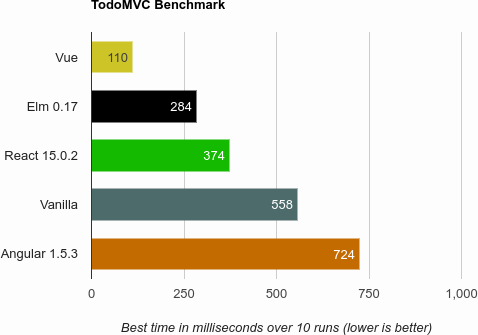
\includegraphics[width=1\textwidth]{img/perf_chromium}
        \caption{Test w przeglądarce Chromium 102.0.5005.61}\label{fig:perf_chromium}
    \end{subfigure}
    \begin{subfigure}{.49\textwidth}
        \centering
        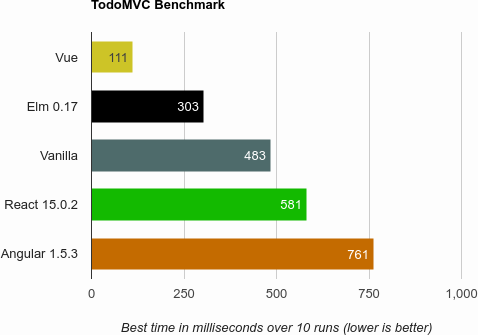
\includegraphics[width=1\textwidth]{img/perf_firefox}
        \caption{Test w przeglądarce Firefox 101.0}\label{fig:perf_firefox}
    \end{subfigure}
    \caption{Testy wydajnościowe aplikacji TodoMVC}\label{fig:perf}
\end{figure}

Można zauważyć, że wyniki różnią się w zależności od użytej przeglądarki internetowej.
W obu przypadkach najszybsza okazała się implementacja w Vue, a najwolniejsza implementacja z użyciem Angulara.
Aplikacja w Elmie uplasowała się na drugim miejscu.
We wszystkich przypadkach aplikacje uruchamiane w przeglądarce Chromium działały szybciej niż w konkurencyjnym Firefoxie.
Największą różnicę można zauważyć w przypadku Reacta, gdzie aplikacja poradziła sobie w Chromium o ok.~35\% lepiej niż w przeglądarce od Mozilli.

\section{Narzędzia}
W kolejnej części pracy chciałbym porównać narzędzia dostępne w Elmie z zestawami narzędzi zalecanymi do pracy z Reactem.

Pierwszą rzeczą, na która od razu zwróciłem uwagę jest różnica w ilości dostępnych narzędzi wspomagających pracę z tymi rozwiązaniami.
Jest to spodziewana sytuacja ze względu na ich rozbieżną popularność --- dużo więcej dostępnych jest zestawów narzędziowych oferujących pomoc do pracy z Reactem niż z Elmem.

Przykładem są narzędzia takie jak~,,Create React App'', które pozwalają na zainicjalizowanie nowego projektu wraz z wygenerowaniem kodu, który spełnia minimalne wymagania do prawidłowego działania aplikacji.
Znacznie przyspiesza to początek pracy nad aplikacją.



\section{Opinia}
Celem tej sekcji jest przedstawienie mojej subiektywnej opinii na temat Elma, biorąc pod uwagę moje doświadczenia zarówno z tym językiem, jak i innymi, z którymi miałem możliwość pracować.

Przed rozpoczęciem pracy nad aplikacją miałem jedynie podstawowe doświadczenie z językami funkcyjnymi, jednakże nauka Elma okazała się bardzo przyjemna.
Oficjalny poradnik języka okazał się być bardzo przydatny i zdecydowanie pomógł mi zrozumieć składnię języka i architekturę tworzenia aplikacji w Elmie.

Całe doświadczenie z językiem oceniam jako bardzo pozytywne.
Wielkim atutem okazał się tutaj kompilator Elma, który dostarczał wnikliwe uwagi na temat pisanego kodu i proponował rozsądne propozycje rozwiązań problemów, jeżeli takie wystąpiły.
Było to szczególnie pożyteczne w przypadku refaktoryzacji kodu, gdzie jako programista nie musiałem się martwić, czy program po wszystkich zmianach będzie dalej działał prawidłowo.
Wystarczyło zastosować się po kolei do wszystkich komunikatów kompilatora i pozwoliło to przeprowadzić efektywną i bezbolesną refaktoryzację.

Jednakże dużym problemem Elma jest częsty brak kompatybilności wstecznej pomiędzy wersjami platformy.
Aplikacje napisane z uzyciem Elma w wersji 0.18 zwyczajnie nie będą działać po aktualizacji kompilatora do wersji 0.19.
Wymaga to dodatkowego nakładu pracy związanego z refaktoryzacją, która jak często wspomniałem jest bezbolesna, jednakowoż czasami potrzebne jest niestety całkowite przepisanie wielu funkcji i szukanie nowych rozwiązań dla powstałych problemów.

% ---------------------------------------------------------------------------------------------------------------------

\chapter{Instrukcja laboratoryjna}
W poniższym rozdziale przedstawiam przykładową instrukcję laboratoryjną, która krok po kroku przeprowadza czytelnika przez proces tworzenia aplikacji w Elmie, zaczynając od przygotowania środowiska deweloperskiego, przez podstawy języka wraz z ćwiczeniami pozwalającymi na lepsze zrozumienie składni, aż po stworzenie większej aplikacji frontendowej.

\section{Przygotowanie środowiska}
Pierwszą rzeczą, którą należy się zająć przed rozpoczęciem nowego projektu jest przygotowanie odpowiedniego środowiska deweloperskiego.
Należy upewnić się, że wszystkie narzędzia potrzebne do wykonania pracy są zainstalowane i prawidłowo skonfigurowane.
W przypadku pracy z Elm'em zalecane będzie korzystanie przede wszystkim z platformy dostarczanej przez autora, edytora tekstu wspierającego podświetlanie składni, a także innych narzędzi wspomagających proces tworzenia oprogramowania z użyciem tej technologii.

\subsection{Platforma Elm}
Najważniejszą rzeczą, jaka będzie potrzebna podczas pracy z Elm'em, będzie platforma języka zawierająca m.in.~takie narzędzia jak kompilator oraz menadżer bibliotek.
Poniżej przedstawiam instrukcję instalacji tej platformy na systemach operacyjnych Linux i Windows.
Po przejściu tych kroków, w wierszu poleceń należy wykonać instrukcję \texttt{elm}.
Jeśli wszystko zostało prawidłowo zainstalowane i skonfigurowane, na ekranie powinien pojawić się widok podobny do przedstawionego na rysunku~\ref{fig:elm_output}.

\begin{figure}[H]
    \centering
    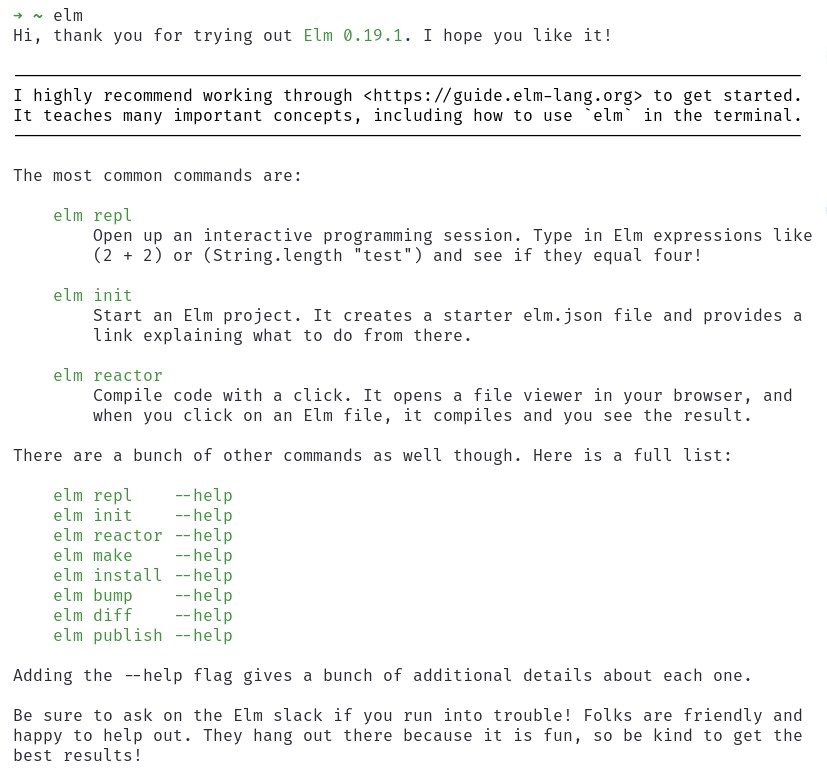
\includegraphics[width=0.95\textwidth]{img/elm_output.png}
    \caption{Wyjście instrukcji \texttt{elm}}\label{fig:elm_output}
\end{figure}

\subsubsection{Linux}
Najprostszym sposobem instalacji platformy Elm na systemie operacyjnym Linux jest wykorzystanie narzędzia \texttt{npm}~-- powszechnie używanego menadżera pakietów służącego do zarządzania warstwą frontendową aplikacji internetowych.
Aby zainstalować \texttt{npm} należy skorzystać z systemowego menadżera pakietów.
Na przykładzie dystrybucji Ubuntu będą to komendy:

\begin{lstlisting}
  $ sudo apt update
  $ sudo apt install npm
\end{lstlisting}

Kiedy narzędzie zostanie już pomyślnie zainstalowane, można przejść do instalacji platformy Elm.
Posłuży do tego polecenie:

\begin{lstlisting}
  $ npm install -g elm
\end{lstlisting}

Zgodnie z dokumentacją \texttt{npm}~\cite{npmdocs}, flaga \texttt{-g} oznacza, że pakiet zostanie zainstalowany globalnie, dzięki czemu będzie dostępny z każdego miejsca z systemu.
Aby sprawdzić, czy rzeczywiście tak się stało, wystarczy w wierszu poleceń uruchomić komendę \texttt{elm}.
Jeżeli wszystkie kroki przebiegły pomyślnie, na ekranie powinien ukazać się widok podobny do przedstawionego na rysunku~\ref{fig:elm_output}, tak jak zostało to już wcześniej wspomniane.

\subsubsection{Windows}
Osoby korzystające z systemu operacyjnego Windows mogą skorzystać z npm, tak jak to było opisane w powyższej sekcji dotyczącej Linuxa lub posłużyć się dedykowanym \href{https://github.com/elm/compiler/releases/download/0.19.1/installer-for-windows.exe}{instalatorem Elm'a}~\cite{elm_installer} na system Windows.
W tym drugim przypadku wystarczy przejść przez wszystkie kroki zostawiając opcje domyślne i w rezultacie Elm zostanie pomyślnie zainstalowany i będzie gotowy do użytkowania.
W celu sprawdzenia czy faktycznie tak się stało, należy uruchomić wiersz poleceń oraz wykonać instrukcję \texttt{elm}.
Wyjście komendy powinno być podobne do tego przedstawionego na rysunku~\ref{fig:elm_output}, tak jak zostało to już wcześniej wspomniane.

\subsection{Edytor}
Ważnym elementem tworzenia oprogramowania jest wyposażenie się w odpowiedni edytor tekstowy, który jest w stanie podświetlać składnię języka, z którego aktualnie korzystamy.
Żeby osiągnąć ten cel, w przypadku Elm'a potrzebna będzie instalacja dodatkowej wtyczki do jednego z następujących edytorów:

\begin{itemize}[noitemsep,topsep=0pt]
    \item{\href{https://atom.io/packages/language-elm}{Atom}}
    \item{\href{https://github.com/jcollard/elm-mode}{Emacs}}
    \item{\href{https://github.com/klazuka/intellij-elm}{IntelliJ}}
    \item{\href{https://github.com/rundis/elm-light}{Light Table}}
    \item{\href{https://github.com/evancz/elm-syntax-highlighting/}{Sublime Text}}
    \item{\href{https://github.com/elm-tooling/elm-vim}{Vim}}
    \item{\href{https://github.com/elm-tooling/elm-language-client-vscode}{VS Code}}
\end{itemize}

Powyższa lista zawiera odnośniki do wspomnianych wtyczek dla danego edytora, wystarczy kliknąć nazwę swojego ulubionego edytora i pobrać odpowiedni dodatek.
Na potrzeby niniejszej instrukcji przedstawię proces instalacji i konfiguracji wtyczki dla edytora Visual Studio Code~\cite{vscode}, ponieważ jest to jedno z najbardziej powszechnie używanych narzędzi do pracy z kodem źródłowym.

// TODO instrukcja vscode

\subsection{Tworzenie projektu}
Elm jest dostarczany wraz z zestawem bardzo przydatnych narzędzi.
Jednym z nich jest \texttt{elm init}, które posłuży nam do stworzenia nowego projektu.
W tym celu należy otworzyć wiersz poleceń i wykonać następujące instrukcje:

\begin{lstlisting}
  $ mkdir lab
  $ cd lab
  $ elm init
\end{lstlisting}

Po wypisaniu zawartości katalogu \texttt{lab} z użyciem polecenia \texttt{ls} powinny pojawić się dwa nowe elementy:

\begin{itemize}[noitemsep,topsep=0pt]
    \item{Plik \texttt{elm.json} opisujący projekt oraz jego zależności}
    \item{Katalog \texttt{src/} zawierający nasze przyszłe pliki Elm'a}
\end{itemize}

Następnym krokiem będzie utworzenie nowego pliku \texttt{Main.elm} w nowo utworzonym katalogu \texttt{src/}.
Będzie się tam znajdował kod aplikacji, która zostanie stworzona w kolejnych krokach.

\section{Podstawy języka Elm}
W celu nauki podstaw języka Elm użyte zostanie narzędzie \texttt{elm repl}, pozwalającego na korzystanie z interaktywnej sesji programistycznej.
Należy otworzyć wiersz poleceń i wpisać polecenie \texttt{elm repl}.
Powinien ukazać się widok podobny do przedstawionego na rysunku~\ref{fig:elm_repl_output} poniżej.

\begin{figure}[H]
    \centering
    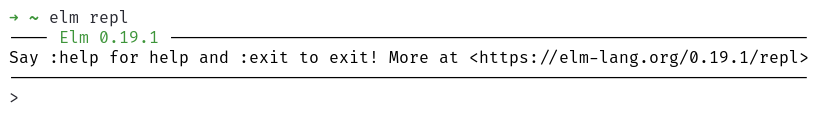
\includegraphics[width=0.95\textwidth]{img/elm_repl_output.png}
    \caption{Otwarta interaktywna sesja \texttt{elm repl}}\label{fig:elm_repl_output}
\end{figure}

\subsection{Wartości}
Najmniejszym budulcem aplikacji w Elmie są \textbf{wartości}.
Mogą to być liczby, ciągi znaków, czy typy logiczne, np. 10,~,,Hello'', True.
Po wpisaniu do okna \texttt{elm repl} danej wartości, na ekranie powinna zostać pokazana powtórzona wartość, a po dwukropku jej typ.

Wartości można także łączyć z operatorami.
Dla liczb będą to typowe operatory matematyczne, jak \texttt{+}, \texttt{-}, \texttt{*}, \texttt{/}, dla ciągów znaków operatorem konkatenacji jest \texttt{++}, a dla typów logicznych dostępne są operatory logiczne~,,\texttt{\&\&}'' (AND) oraz~,,\texttt{||}'' (OR).

Na rysunku~\ref{fig:repl_values} pokazane zostały przykłady efektów takich wywołań.

\begin{figure}[H]
    \centering
    \begin{subfigure}{.29\textwidth}
        \centering
        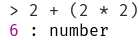
\includegraphics[height=1cm]{img/repl_number}
        \caption{Liczba}\label{fig:repl_number}
    \end{subfigure}
    \begin{subfigure}{.4\textwidth}
        \centering
        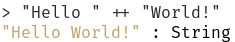
\includegraphics[height=1cm]{img/repl_string}
        \caption{Ciąg znaków}\label{fig:repl_string}
    \end{subfigure}
    \begin{subfigure}{.29\textwidth}
        \centering
        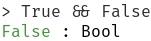
\includegraphics[height=1cm]{img/repl_bool}
        \caption{Typ logiczny}\label{fig:repl_bool}
    \end{subfigure}
    \caption{Wartości w Elmie}\label{fig:repl_values}
\end{figure}

\subsection{Funkcje}
\begin{wrapfigure}{r}{0.45\textwidth}
    \centering
    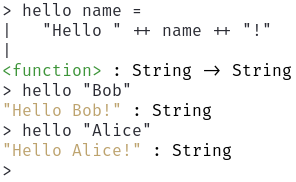
\includegraphics[width=0.45\textwidth]{img/repl_func}
    \caption{Definicja funkcji w Elmie}\label{fig:repl_func}
\end{wrapfigure}

Funkcje w Elmie określają, w jaki sposób wartości mogą zostać przetworzone.
Na rysunku~\ref{fig:repl_func} pokazana została przykładowa funkcja \texttt{hello}, która przyjmuje argument \texttt{name} i zwraca nowy ciąg znaków.

Można zauważyć, że typ argumentu \texttt{name} nie został sprecyzowany.
Elm sam potrafi określić, czy dana funkcja wykona się poprawnie na podstawie operacji w niej zawartych.
W pokazanym przykładzie argument \texttt{name} jest wykorzystany jako operand operatora konkatenacji~,,\texttt{++}'', który potrzebuje dwóch operandów typu \texttt{String} do prawidłowego działania programu.
Jeśli użytkownik zamiast ciągu znaków podałby jako argument inny typ, np.~liczbę, to kompilator Elma zwróciłby na to uwagę i wystosował użytkownikowi odpowiedni komunikat.

Przykład takiego komunikatu został przedstawiony na rysunku~\ref{fig:repl_error}.

\begin{figure}[H]
    \centering
    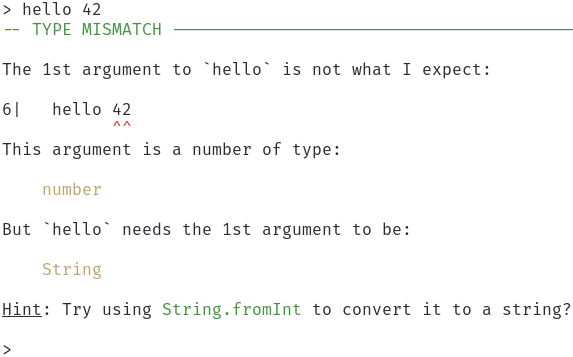
\includegraphics[width=0.7\textwidth]{img/repl_error}
    \caption{Komunikat kompilatora o błędzie}\label{fig:repl_error}
\end{figure}

\subsection{Listy}
Listy są jednymi z najczęściej używanych struktur danych w Elmie.
Ich przeznaczeniem jest trzymanie sekwencji wielu elementów tego samego typu.

Na rysunku~\ref{fig:repl_lists} zostały pokazane przykłady użycia list. Została zdefiniowana lista \texttt{names}, zawierająca trzy elementy typu \texttt{String}, a także tablica \texttt{numbers}, która zawiera 4 liczby (typ \texttt{Int}).

\begin{figure}[H]
    \centering
    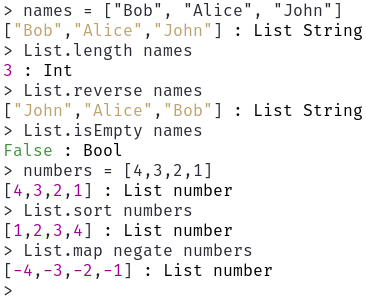
\includegraphics[width=0.5\textwidth]{img/repl_lists}
    \caption{Operacje na listach}\label{fig:repl_lists}
\end{figure}

\subsection{Rekordy}
Rekordy służą do trzymania wielu wartości, gdzie każda z nich jest przypisana do konkretnej nazwy. Na rysunku~\ref{fig:repl_records} pokazane zostały przykładowe operacje związane z rekordami. Zdefiniowany został rekord \texttt{bob}, który zawiera informacje o imieniu, nazwisku oraz wieku.

\begin{figure}[H]
    \centering
    \begin{subfigure}{0.7\textwidth}
        \centering
        \caption{Definicja rekordu i dostęp do jednego z pól}\label{fig:repl_record_bob}
        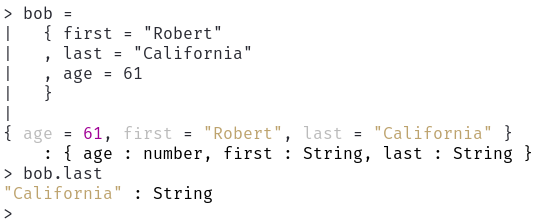
\includegraphics[width=1\textwidth]{img/repl_record_bob}
    \end{subfigure}
    \begin{subfigure}{.7\textwidth}
        \centering
        \caption{Nadpisanie zawartości rekordu}\label{fig:repl_record_update}
        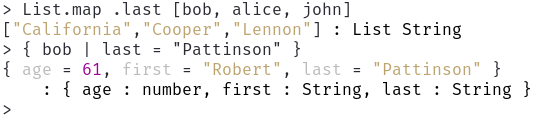
\includegraphics[width=1\textwidth]{img/repl_record_update}
    \end{subfigure}
    \caption{Przykłady pracy z rekordami}\label{fig:repl_records}
\end{figure}

W przypadku rekordów, które zawierają wiele pól, praca z nimi może stawać się problematyczna.
Wygodne może być wtedy wykorzystanie tzw.~,,aliasów typów'', które pozwalają na definicję typu rekordu i korzystanie z niego w skróconej wersji.

Na rysunku~\ref{fig:repl_type_alias} zdefiniowany został nowy typ \texttt{Person}, który jest równoznaczny ze zdefiniowanym na rys.~\ref{fig:repl_record_bob} rekordem \texttt{bob}.
Jednakże tak zdefiniowany typ sprawia, że kod staje się krótszy, bardziej czytelny, a praca z nim dużo wygodniejsza.
\begin{figure}[H]
    \centering
    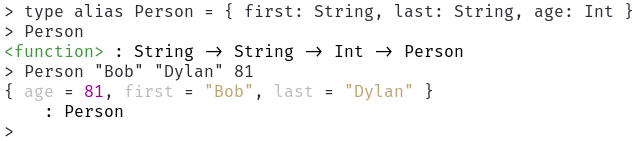
\includegraphics[width=0.85\textwidth]{img/repl_type_alias}
    \caption{Definicja aliasu typu \texttt{Person}}\label{fig:repl_type_alias}
\end{figure}

\section{Aplikacja frontendowa}
W ramach większego projektu zbudowana zostanie strona internetową typu \texttt{startpage}, czyli strona startowa przeglądarki zawierająca najważniejsze i najczęściej używane elementy.
Zaimplementowane zostaną cztery moduły --- Data i czas, pogoda, wyszukiwarka oraz pasek zakładek.

Każda z funkcjonalności będzie dodawana inkrementalnie poprzez dokładanie kolejnych fragmentów kodu do każdej z części architektury Elma, tj. \texttt{Model}, \texttt{Update} oraz \texttt{View}, czyli elementów odpowiedzialnych odpowiednio za stan, logikę i wygląd aplikacji.

Plik źródłowy \texttt{Main.elm} został stworzony w jednym z poprzednich kroków --- należy go otworzyć w swoim wybranym edytorze i przejść do kolejnych kroków.

\subsection{Szkielet aplikacji}
W pierwszej kolejności należy uruchomić aplikację typu~,,Hello World!'', aby upewnić się, że środowisko zostało prawidłowo skonfigurowane.
W załączonym pliku \texttt{Main.elm} znajdują się wszystkie potrzebne do działania klauzule importujące biblioteki podstawowe Elma.
Ponadto zaimplementowana została podstawowa architektura aplikacji.
Aby uruchomić aplikację~,,Hello, World!'' należy otworzyć wiersz poleceń i wykonać polecenie:

\begin{lstlisting}
  $ elm reactor
\end{lstlisting}

Powinien pokazać się następujący widok:

\begin{figure}[H]
    \centering
    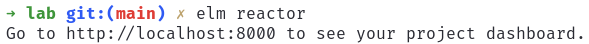
\includegraphics[width=0.9\textwidth]{img/elm_reactor}
\end{figure}

Po otwarciu w przeglądarce adresu \texttt{http://localhost:8000} należy znaleźć plik \texttt{Main.elm} i go otworzyć.
Powinien wyświetlić się napis~,,Hello, World!'' oraz guzik \texttt{Click me!}, który zamienia ciąg tekstowy na~,,Hello, again!''.

Celem dalszych sekcji będzie rozwinięcie tego programu poprzez implementację wymaganych funkcjonalności omówionych na początku instrukcji.

\subsection{Czas}
Do wydobycia informacji o aktualnym czasie wykorzystana zostanie biblioteka \texttt{elm/time}.
W celu zainstalowania tej biblioteki w wierszu poleceń należy wykonać komendę \texttt{\$ elm install elm/time}, a następnie załączyć bibliotekę do tworzonego programu używając klauzuli \texttt{import Time exposing (..)}.

Przechodząc do edycji kodu, pierwszą rzeczą jest zdefiniowanie modelu programu.
Potrzebne będą informacje o strefie czasowej oraz aktualny czas.
W tym celu należy stworzyć nowy typ \texttt{DateTime}, który będzie przechowywał te dane, a następnie dodać go do modelu.

\begin{lstlisting}[language=Elm]
type alias Model =
    { dateTime : DateTime }
type alias DateTime =
    { zone : Time.Zone
    , time : Time.Posix
    }
\end{lstlisting}

Kolejnym krokiem będzie zdefiniowanie typów wiadomości, które może odebrać program.
Do prawidłowego działania zegara potrzebne będzie dostosowanie strefy czasowej oraz pobranie aktualnego czasu.
Oznacza to, że należy zdefiniować dwie wiadomości --- \texttt{AdjustTimeZone} oraz \texttt{Tick}.

\begin{lstlisting}[language=Elm]
type Msg
    = Tick Time.Posix
    | AdjustTimeZone Time.Zone
\end{lstlisting}

Oba typy wiadomości muszą zostać odpowiednio przetworzone w funkcji \texttt{update}.
W obu przypadkach wystarczające będzie nadpisanie stworzonego modelu nowymi wartościami.
Przykład nadpisania rekordu został przedstawiony wcześniej na rys.~\ref{fig:repl_record_update}.

Następnie należy zdefiniować funkcję \texttt{init}, gdzie wskazany zostanie sposób inicjalizacji modelu oraz operacje, jakie mają zostać wykonane na początku programu.
W przypadku daty i czasu należy początkowo wyzerować obie wartości, a następnie pobrać aktualne informacje wykorzystując stworzone przed chwilą wiadomości.

\begin{lstlisting}[language=Elm]
init _ =
    ( Model (DateTime Time.utc (Time.millisToPosix 0))
    , Cmd.batch [ Task.perform AdjustTimeZone Time.here, Task.perform Tick Time.now ]
    )
\end{lstlisting}

Jednakże czas zmienia się z sekundy na sekundę, więc jednorazowe ustawienie wartości modelu niestety nie jest wystarczające --- trzeba aktualizować model co sekundę.
Aby to osiągnąć, wykorzystana zostanie funkcja \texttt{subscriptions}.
Pozwala na nasłuchiwanie zewnętrznych zdarzeń, takich jak kliknięcie myszki, naciśnięcie klawisza na klawiaturze, zmiany w geolokacji lub --- tykanie zegara.

W przypadku tworzonej aplikacji należy co sekundę generować nową wiadomość \texttt{Tick}, która po jej przetworzeniu w funkcji \texttt{update} zaktualizuje aktualny czas w modelu.

\begin{lstlisting}[language=Elm]
subscriptions _ =
    Time.every 1000 Tick
\end{lstlisting}

Ostatnim elementem architektury Elma jest funkcja \texttt{view}, której zadaniem jest wyświetlanie programu na ekranie.

\begin{lstlisting}[language=Elm]
view model =
    { title = "Hello"
    , body =
        [ viewTime model.dateTime
        , viewDate model.dateTime
        ]
    }
\end{lstlisting}

W celu polepszenia czytelności kodu, funkcja \texttt{view} wykorzystuje dwie funkcje pomocnicze --- \texttt{viewTime} oraz \texttt{viewDate}.
Część implementacji jednej z nich została przedstawiona poniżej.
W ramach ćwiczenia należy dokończyć implementację funkcji \texttt{viewDate} oraz stworzyć analogiczną funkcję \texttt{viewTime}.
Ponadto przedstawiony został początek funkcji \texttt{toEnglishWeekday}, która przyjmuje wartość typu \texttt{Time.Weekday} i zwraca typ \texttt{String}, który może zostać następnie wyświetlony w funkcji \texttt{viewDate}.
Implementację tej funkcji także należy dokończyć oraz stworzyć analogiczną funkcję pozwalającą na dekodowanie nazw miesięcy.
Dla lepszego wyglądu zegara warto także stworzyć funkcję dodającą znak 0 dla liczb mniejszych od 10.
\begin{lstlisting}[language=Elm]
viewDate dateTime =
    let
        weekday =
            Time.toWeekday dateTime.zone dateTime.time
        ...
    in
    div [] [ text (toEnglishWeekday weekday) ]
toEnglishWeekday weekday =
    case weekday of
        Mon ->
            "Monday"
        ...
\end{lstlisting}

Jeżeli wszystko udało się pomyślnie, w przeglądarce internetowej powinien wyświetlić się aktualny czas, zmieniający się co sekundę, a pod nim data.
Następnie można przejść do kolejnej sekcji.

\subsection{Pogoda}
Pogoda będzie pobierana wykorzystując zapytania HTTP do API portalu OpenWeatherMap\@.
Potrzebne będą do tego dwie biblioteki --- \texttt{elm/http} do wysłania zapytania oraz \texttt{elm/json} do odebrania i przetworzenia odpowiedzi w formacie JSON\@.
Podobnie jak poprzednio, należy je zainstalować używając poleceń:
\begin{lstlisting}
  $ elm install elm/http
  $ elm install elm/json
\end{lstlisting}
Następnie należy dodać do pliku \texttt{Main.elm} następujące klauzule:

\begin{lstlisting}[language=Elm]
import Http
import Json.Decode exposing (..)
\end{lstlisting}

Przed przejściem do edycji kodu programu należy założyć darmowe konto na stronie \href{https://openweathermap.org/}{OpenWeatherMap}, a następnie wygenerować klucz API, który będzie konieczny do prawidłowego działania aplikacji.
Po stworzeniu prywatnego klucza API można przejść do kolejnych kroków.

W przypadku pogody potrzebne będzie stworzenie dwóch nowych typów: jeden będzie zawierał informacje o faktycznym stanie pogody, tj.~temperatura i krótki opis słowny, a drugi informacje o statusie zapytania HTTP\@.

\begin{lstlisting}[language=Elm]
type WeatherStatus
    = Failure String
    | Loading
    | Success Weather
type alias Weather =
    { description : String
    , temperature : Float
    }
\end{lstlisting}

Powyższy typ \texttt{WeatherStatus} należy dodać do głównego modelu.
Ponadto należy zdefiniować w programie dane potrzebne do wysłania zapytania, a następnie wykorzystać je w funkcji odpowiedzialnej za wysłanie zapytania GET do OpenWeatherAPI\@.
Są to:
\begin{itemize}[noitemsep,topsep=0pt]
    \item URL do wysłania zapytania
    \item Prywatny klucz API do OpenWeatherMap
    \item Miasto
    \item Jednostki
\end{itemize}
Przykład implementacji został przedstawiony poniżej:

\begin{lstlisting}[language=Elm]
getWeather =
  Http.get
    { url = weatherApi ++ ("&q=" ++ city) ++ ("&units=" ++ unit) ++ ("&appid=" ++ apiKey)
    , expect = Http.expectJson GotWeather weatherDecoder
    }
\end{lstlisting}
Szczegóły użycia API opisane są w \href{https://openweathermap.org/current#name}{dokumentacji OpenWeatherMap}.

Z perspektywy Elma najważniejsze jest sprecyzowanie rodzaju zapytania (tutaj GET) oraz adresu URL, na który ma został wysłane zapytanie.
Konieczne jest także określenie formy spodziewanej odpowiedzi (JSON), a także przekazanie funkcji jej dekodującej.
Na końcu należy przekazać rodzaj wiadomości do wygenerowania po odebraniu odpowiedzi (\texttt{GotWeather}).

A jak wygląda funkcja i dekodująca i do czego służy?
Przykład prostego dekodera został przedstawiony poniżej.
Celem dekodera jest przetworzenie pliku w formacie JSON w taki sposób, aby był zrozumiały dla Elma.
Należy w nim określić nazwy oczekiwanych pól oraz opisać jak się do nich dostać.

Funkcja \texttt{personDecoder} spodziewa się trzech wartości --- dwóch ciągów znaków i jednej liczby, które znajdują się w polach nazwanych odpowiednio \texttt{first}, \texttt{last} oraz \texttt{age}.
Typ \texttt{Person} został stworzony na rys.~\ref{fig:repl_record_update} i zawiera w sobie takie same typy jak dekoder.
Oznacza to, że taka odpowiedź JSON powinna zostać prawidłowo zmapowana na typ \texttt{Person}.
\begin{lstlisting}[language=Elm]
personDecoder =
  map3 Person
      (field "first" string)
      (field "last" string)
      (field "age" int)
\end{lstlisting}

W ramach ćwiczenia należy zaimplementować funkcję \texttt{weatherDecoder}, która zmapuje odpowiednie pola z odpowiedzi JSON na typ \texttt{Weather} zaimplementowany wcześniej w modelu.

W przypadku wiadomości \texttt{Msg} sytuacja będzie podobna jak przy tworzeniu typów --- potrzebny będzie jeden rodzaj wiadomości odpowiedzialny za wysłanie zapytania oraz drugi odpowiedzialny za jego odebranie i odpowiednie zaktualizowanie modelu na podstawie danych odebranych z dekodera.

\begin{lstlisting}[language=Elm]
type Msg
    = ...
    | UpdateWeather
    | GotWeather (Result Http.Error Weather)
\end{lstlisting}

\begin{lstlisting}[language=Elm]
update msg model =
  case msg of
    ...
    UpdateWeather ->
      ( { model | weatherStatus = Loading }, getWeather )
    GotWeather result ->
      case result of
        Ok weather ->
          ( { model | weatherStatus = Success weather }, Cmd.none )
        Err _ ->
          ( { model | weatherStatus = Failure "Error: Couldn't retrieve weather data" }, Cmd.none)
\end{lstlisting}


\subsection{Wyszukiwarka}
Wyszukiwarka jest jedną z prostszych funkcjonalności do implementacji.
Potrzebne będzie jedynie stworzenie pola tekstowego, gdzie użytkownik może wpisać wybraną frazę, oraz jego odpowiednie obsłużenie.
Po wpisaniu frazy i wciśnięciu klawisza Enter użytkownik powinien zostać przeniesiony do strony wyszukiwarki z wyszukanym wpisanym już wcześniej hasłem.

Można zauważyć, że tym razem do modelu należy dołożyć jedynie jedną wartość --- ciąg znaków wpisany przez użytkownika.
Wiadomości typu \texttt{Msg} natomiast będą dwie --- jedna standardowo odpowiedzialna za zaktualizowanie modelu, a druga za przekierowanie strony do wyszukiwarki.
Przekierowanie odbywa się za pomocą funkcji \texttt{load} z biblioteki \texttt{Navigation}, która powinna już być załączona do programu w początkowym szkielecie.
Poniżej zostały przedstawione propozycje implementacji wiadomości \texttt{Search} obsługującej przekierowanie do wyszukiwarki oraz funkcji \texttt{viewSearchBar} wyświetlającej pole tekstowe.
Dodatkowo zaimplementowana została funkcja \texttt{onEnter} pozwalająca na wykrycie czy użytkownik wcisnął klawisz Enter.
\begin{lstlisting}[language=Elm]
Search ->
  ( model
  , Nav.load ("https://google.com/search?q=" ++ model.searchText)
  )
\end{lstlisting}
\begin{minipage}{.56\textwidth}
\begin{lstlisting}[language=Elm]
onEnter msg =
  let
    isEnter code =
      if code == 13 then
        succeed msg
      else
        fail "not ENTER"
  in
  on "keydown" (andThen isEnter keyCode)
\end{lstlisting}
\end{minipage}\hfill
\begin{minipage}{.38\textwidth}
\begin{lstlisting}[language=Elm]
viewSearchBar =
  div []
    [ input
      [ type_ "text"
      , placeholder "Search"
      , onInput UpdateField
      , onEnter Search
      ] []
    ]
\end{lstlisting}
\end{minipage}\hfill

W ramach ćwiczenia należy zaimplementować model oraz rozszerzyć funkcję \texttt{update} o dwie nowe wiadomości, jak i główną funkcję \texttt{view} o przedstawioną wyżej propozycję \texttt{viewSearchBar}.
Po prawidłowym złączeniu wszystkich fragmentów kodu program powinien się kompilować i wyświetlać nowy pasek pola tekstowego, a po wciśnięciu klawisza Enter strona powinna zostać przekierowana do wyszukiwarki Google.

Jeżeli wszystko udało się zaimplementować pomyślnie, można przejść do kolejnego kroku.

\subsection{Zakładki}
W dalszej części implementacji
Do prawidłowego działania zakładek potrzebne będzie stworzenie dwóch dodatkowych plików --- \texttt{bookmarks.js} oraz \texttt{index.html}.
Pierwszy posłuży do trzymania listy zakładek, gdzie każda składa się z adresu URL oraz nazwy, która zostanie wyświetlona na tworzonej stronie.
Natomiast drugi plik \texttt{index.html} potrzebny będzie do załadowania do programu poprzedniego pliku z zakładkami jak i pliku wynikowego stworzonego przez kompilator Elma z użyciem następującej komendy:
\begin{lstlisting}
  $ elm make src/MainBookmarks.elm --output=assets/elm.js
\end{lstlisting}

W sekcji \texttt{<head>} pliku \texttt{index.html} należy załączyć plik z zakładkami oraz wynikowy plik kompilatora.
W sekcji \texttt{<body>} należy dodać fragment kodu przedstawiony poniżej, który pozwoli na wykorzystanie programu w Elmie razem z zewnętrznym plikiem HTML\@.

\noindent
\begin{minipage}{.41\textwidth}
\begin{lstlisting}[language=html]
<head>
  <script
    src="assets/elm.js">
  </script>
  <script
    src="assets/bookmarks.js">
  </script>
</head>
\end{lstlisting}
\end{minipage}\hfill
\begin{minipage}{.55\textwidth}
\begin{lstlisting}[language=html]
<body>
  <div id="app"></div>
  <script>
    var app = Elm.Main.init({
      node: document.getElementById("app"),
      flags: bookmarks,
    });
  </script>
</body>
\end{lstlisting}
\end{minipage}\hfill

Po otwarciu pliku \texttt{index.html} z użyciem programu \texttt{elm reactor} aplikacja wraz z zakładkami powinna pojawić się na ekranie.

\subsection{Style}
W załączonym pliku \texttt{styles.css} znajdują się kaskadowe arkusze stylów, które mogą zostać wykorzystane wraz ze stworzoną aplikacją.
W tym celu należy odpowiednio zmienić w programie funkcje odpowiedzialne za wyświetlanie elementów, dodając do nich tagi \texttt{div[][]}.
Funkcja \texttt{div} przyjmuje dwa argumenty: listę atrybutów oraz listę elementów HTML\@.
W tej części należy skupić się na pierwszym argumencie, gdyż dotychczas nie był on jeszcze używany.
Atrybuty HTML to np. \texttt{class}, \texttt{id} oraz \texttt{style}.

Na przykładzie głównej funkcji \texttt{view}, wykorzystanie klasy \texttt{container} wygląda następująco:
\begin{lstlisting}[language=Elm]
view model =
  { ...
  , body =
    [ div [ class "container" ]
      [ viewTime model.clockTime
        ... ] ]
  }
\end{lstlisting}

Jako, że plik \texttt{styles.css} został dostarczony w załączniku, w ramach ćwiczenia w aplikacji wystarczy jedynie dodać w odpowiednich miejscach funkcje \texttt{div} wraz z pasującymi atrybutami, które zostały zdefiniowane w arkuszu stylów.

\subsection{Efekt}
Jeżeli wszystkie funkcjonalności zostały prawidłowo zaimplementowane, a arkusze stylów właściwie użyte w programie, finalna aplikacja powinna wyglądać następująco:
\begin{figure}[H]
    \centering
    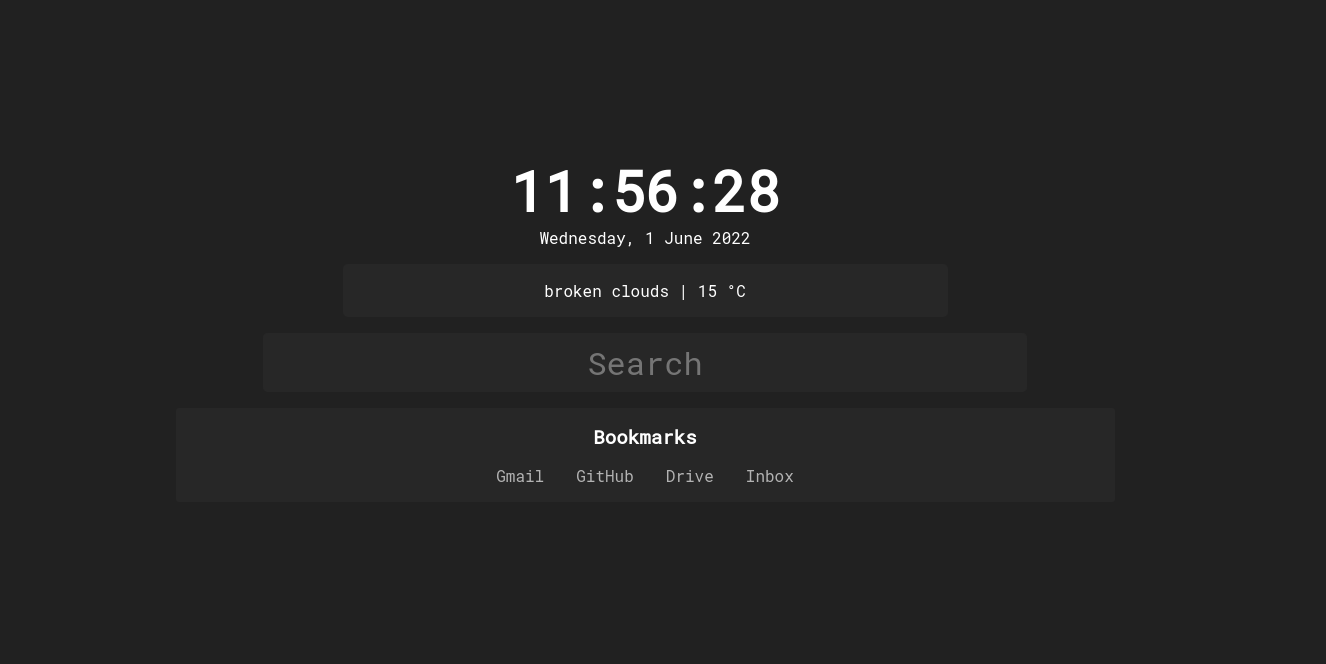
\includegraphics[width=0.9\textwidth]{img/final_app.png}
\end{figure}

% ---------------------------------------------------------------------------------------------------------------------

\chapter{Automatyzacja}
W poniższym rozdziale chciałbym opisać procesy CI/CD oraz korzyści płynące z ich użytkowania, a także zaprezentować implementację takiego rozwiązania na przykładzie stworzonej wcześniej aplikacji w Elm'ie.

\section{CI/CD}
Mianem CI/CD określa się zbiór praktyk pozwalających na ciągłą integrację oraz ciągłe dostarczanie projektów informatycznych.
\begin{figure}[H]
    \centering
    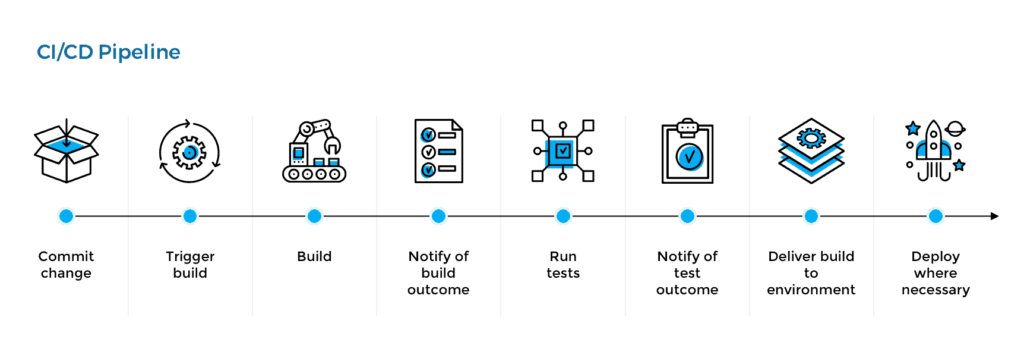
\includegraphics[width=1\textwidth]{img/cicd_pipeline.png}
    \caption{Przykładowy potok CI/CD}\label{fig:cicd_pipeline}
\end{figure}
Na rysunku~\ref{fig:cicd_pipeline} przedstawiony został przykład potoku CI/CD\@.
Jego kroki zostaną omówione w kolejnych podrozdziałach.

\subsection{Ciągła integracja}
,,Ciągłą integracją'' (CI) nazywa się praktyki wykorzystywane przy tworzeniu oprogramowania, polegające na regularnym kontrybuowaniu do zdalnego repozytorium kodu przez zespół deweloperski, gdzie za każdym razem następuje weryfikacja wprowadzonych zmian.
Dzieje się to poprzez automatyczne budowanie projektu oraz wykonanie testów jednostkowych, a na końcu udostępnienie artefaktów

Korzyści wynikające z używania ciągłej integracji obejmują między innymi:
\begin{itemize}[noitemsep,topsep=0pt]
    \item wczesne wykrywanie błędów
    \item zmniejszenie kosztów i ilości pracy manualnej
\end{itemize}

Na rynku dostępnych jest wiele narzędzi oferujących usługi wspierające CI\@. Kilka najpopularniejszych z nich to m.in. Jenkins, TeamCity i CircleCI\@.
Są to potężne narzędzia, umożliwiające tworzenie i zarządzanie potokami ciągłej integracji nawet w przypadku bardzo rozbudowanych projektów prowadzonych przez największe firmy informatyczne.

Ciągła integracja skupia się głównie na pracy zespołu deweloperskiego i to właśnie jego dotyczy informacja zwrotna przekazywana przez wyniki potoku.
Mogą to być błędy kompilacji, problemy z łączeniem gałęzi repozytorium (\textit{merge conflicts}) czy wskazanie testów, które zakończyły się niepowodzeniem.

Martin Fowler w swojej książce~,,Continuous Integration''~\cite{fowler2006continuous} przedstawia i opisuje następujące praktyki:
\begin{itemize}[noitemsep,topsep=0pt]
    \item Utrzymuj jedno repozytorium kodu --- systemy kontroli wersji są integralną częścią większości projektów deweloperskich. Repozytorium powinno zawierać wszystkie pliki źródłowe i każdy członek zespołu powinien mieć do niego dostęp.
    \item Zautomatyzuj budowanie projektu --- często jest to skomplikowany proces, jednak jak większość zadań w procesie deweloperskim może zostać zautomatyzowany, i w rezultacie powinien.
    \item Przygotuj testy --- pozwala to bardzo szybko i efektywnie wychwycić błędy, szczególnie jeśli będą uruchamiane przy każdym budowaniu projektu.
    \item Każdy deweloper codziennie nanosi zmiany w głównej gałęzi --- codzienne zmiany, które są automatycznie budowane i testowane pozwalają na szybkie wykrycie błędów, nawet tych potencjalnych, które mogą wynikać z konfliktu pracy dwóch deweloperów.
    \item Każda zmiana powinna zostać zbudowana na maszynie integracyjnej --- zmiana jest uznana za~,,gotową'' dopiero wtedy, gdy powiedzie się na maszynie integracyjnej.
    \item Naprawiaj nieudane buildy natychmiastowo --- głównym zamysłem ciągłej integracji jest praca na stabilnej gałęzi repozytorium. Jeżeli budowa projektu się nie powiodła, naprawienie zmian powinno być najważniejszym i najpilniejszym zadaniem do wykonania.
    \item Budowa ma odbywać się szybko --- ciągła integracja ma zapewniać błyskawiczną informację zwrotną. Czas jest mocno zależny od danego projektu, ale 10--15 minutowa budowa projektu jest uznawana za odpowiednią długość.
    \item Testuj w odpowiedniku środowiska produkcyjnego --- celem testów jest upewnienie się, że system działa prawidłowo w docelowym środowisku, więc uruchamianie ich w środowisku innym niż produkcyjne mija się z celem.
    \item Ułatw dostęp do ostatnich plików wynikowych --- po zakończeniu budowania wszystkie artefakty powinny być dostępne do pobrania.
    \item Wszyscy widzą co się dzieje --- użytkownicy ciągłej integracji powinni mieć możliwość zobaczenia co się dzieje w systemie. Oznacza to wprowadzenie znaczników określających, czy dany build się powiódł.
\end{itemize}

\subsection{Ciągłe dostarczanie}
,,Ciągłe dostarczanie'' to praktyka pozwalająca na automatyzację procesu dostarczania (publikowania) oprogramowania na podstawie nowych artefaktów kompilacji.
Oznacza to, że jest ściśle związana z ciągłą integracją, której założeniem jest posiadanie jednej głównej gałęzi w repozytorium kodu, która jest zawsze stabilna i gotowa do publikacji.

Skrót \textit{CD} powoduje nieraz pewne zamieszanie, gdyż często używany jest zamiennie dla dwóch pojęć --- ciągłego dostarczania oraz ciągłego wdrażania.
Są to procesy bardzo zbliżone, gdyż oba polegają na automatyzacji procesu dostarczania oprogramowania do środowiska produkcyjnego.
Różnica polega na tym, że ciągłe dostarczanie wymaga ręcznej interakcji człowieka, który określi kiedy ma zostać wykonane wdrożenie, gdzie w ciągłym wdrażaniu cały proces dzieje się automatycznie, bez wpływu człowieka.

W praktyce ciągłe wdrażanie jest zdecydowanie rzadziej spotykane, gdyż pełna automatyzacja, obejmująca m.in.~testy integracyjne, wydajnościowe i akceptacyjne, jest niesamowicie trudna do osiągnięcia.

\section{GitHub Actions}
Od samego rozpoczęcia pracy nad aplikacją w Elmie, cały kod źródłowy przechowywany był z użyciem systemu kontroli wersji Git~\cite{git}, a wybór serwisu hostującego zdalne repozytorium kodu padł na GitHub~\cite{github}.
Ze względu na ten wybór jak i niewielki rozmiar stworzonej w Elmie aplikacji, zdecydowałem się wykorzystać GitHub Actions do zbudowania potoków CI/CD\@.

W odróżnieniu od standardowych przypadków użycia potoków CI/CD, gdzie oprogramowanie jest tworzone przez zespół deweloperski składający się z wielu osób, aplikacja powstała w ramach niniejszej pracy magisterskiej została stworzona przez jedną osobę.
Jest to specyficzny przypadek, gdyż w takiej sytuacji nie ma możliwości wystąpienia problemów, które często mogą pojawić się w zespołach deweloperskich podczas próby integracji, na przykład konflikty łączenia gałęzi.

Jednakże, celem mojej implementacji było pokazanie, że techniki CI/CD mogą zostać efektywnie wykorzystane podczas pracy z językiem Elm.

Zaimplementowany potok CI/CD dla aplikacji w Elmie został przedstawiony na rys.~\ref{fig:elm_yml}.
Składa się z kroku \textit{build}, którego celem jest przygotowanie środowiska, tj.~instalacja platformy Elm oraz pobranie kodu źródłowego, a następnie zbudowanie aplikacji i udostępnienie artefaktu kompilacji oraz z kroku \textit{deploy}, który przygotowuje oddzielną gałąź \textit{gh-pages} poprzez pobranie i aktualizację udostępnionego wcześniej pliku wynikowego.
\begin{figure}[H]
    \centering
    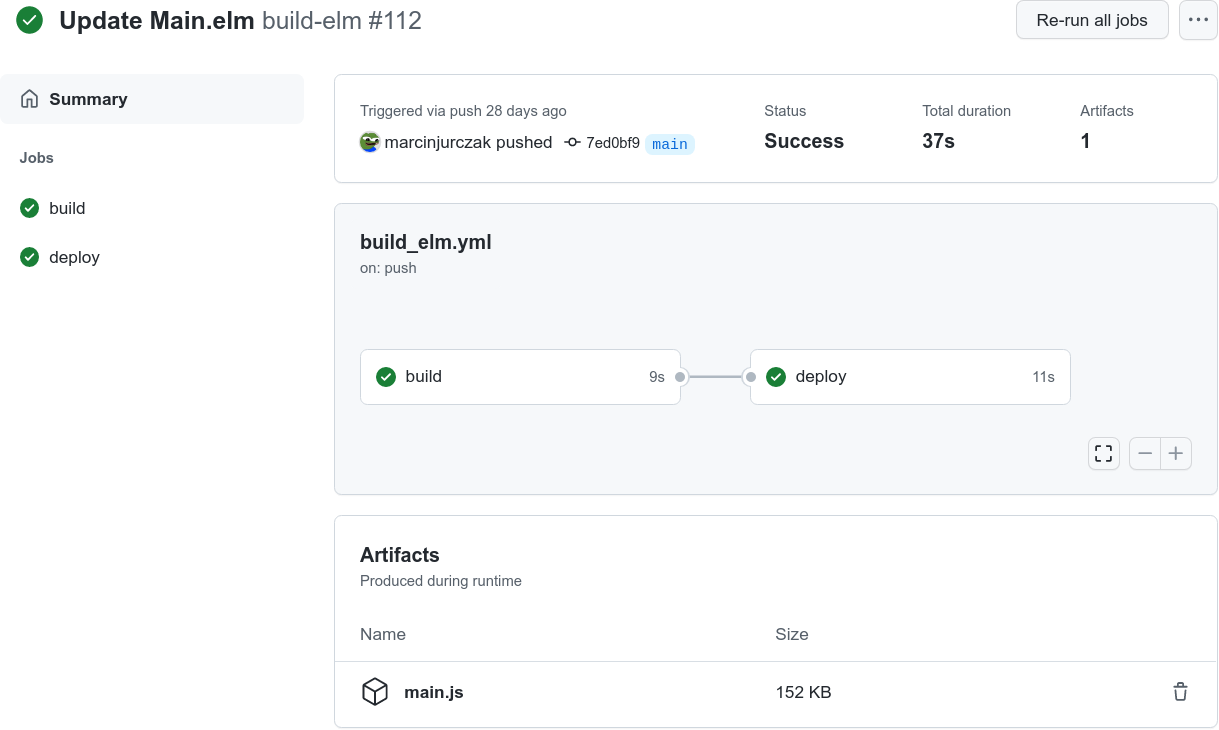
\includegraphics[width=0.95\textwidth]{img/elm_yml.png}
    \caption{Widok CI/CD aplikacji w Elmie}\label{fig:elm_yml}
\end{figure}

Następnie przygotowana gałąź zostaje wystawiona przez GitHub Pages, co zostanie szczegółowiej opisane w kolejnej sekcji.

\section{GitHub Pages}
Serwis GitHub udostępnia możliwość hostowania stron internetowych prosto z repozytorium kodu. Warto zaznaczyć, że ta opcja jest dostępna za darmo, pod warunkiem, że hostowana strona znajduje się w \textbf{publicznym} repozytorium kodu. Aby skorzystać z usług GitHub Pages dla prywatnego repozytorium konieczne jest wykupienie jednej z płatnych opcji.

Wykorzystanie funkcjonalności Pages jest dość proste --- w ustawieniach repozytorium należy ustawić gałąź (\textit{branch}), która ma zostać wystawiona na stronie, a także wybrać odpowiedni katalog.
Domyślnie mogą być to jedynie katalogi \texttt{/} (\texttt{root}) oraz \texttt{/docs}.

Jednakże wykorzystując GitHub Actions możliwe jest bardziej szczegółowe dostosowanie tej strony do swoich potrzeb.
W przypadku stworzonej w ramach tej pracy aplikacji w Elmie, kod źródłowy znajdował się w podkatalogu \texttt{/elm}.
W wyniku stworzonej konfiguracji, na gałęzi \texttt{gh-pages} zostaje opublikowana aktualna zawartość katalogu \texttt{/elm}, a następnie do tej samej gałęzi dodawany jest otrzymany podczas przeprowadzonej w poprzednim kroku fazy budowania wynikowy plik \texttt{main.js}.
GitHub Pages znajduje w wybranym miejscu plik \texttt{index.html}, który zostaje wystawiony i strona staje się dostępna do oglądania w Internecie.

Na rysunku~\ref{fig:deploy_yml} został zaprezentowany domyślny widok potoku pozwalającego na publikację aplikacji z użyciem GitHub Pages.
\begin{figure}[H]
    \centering
    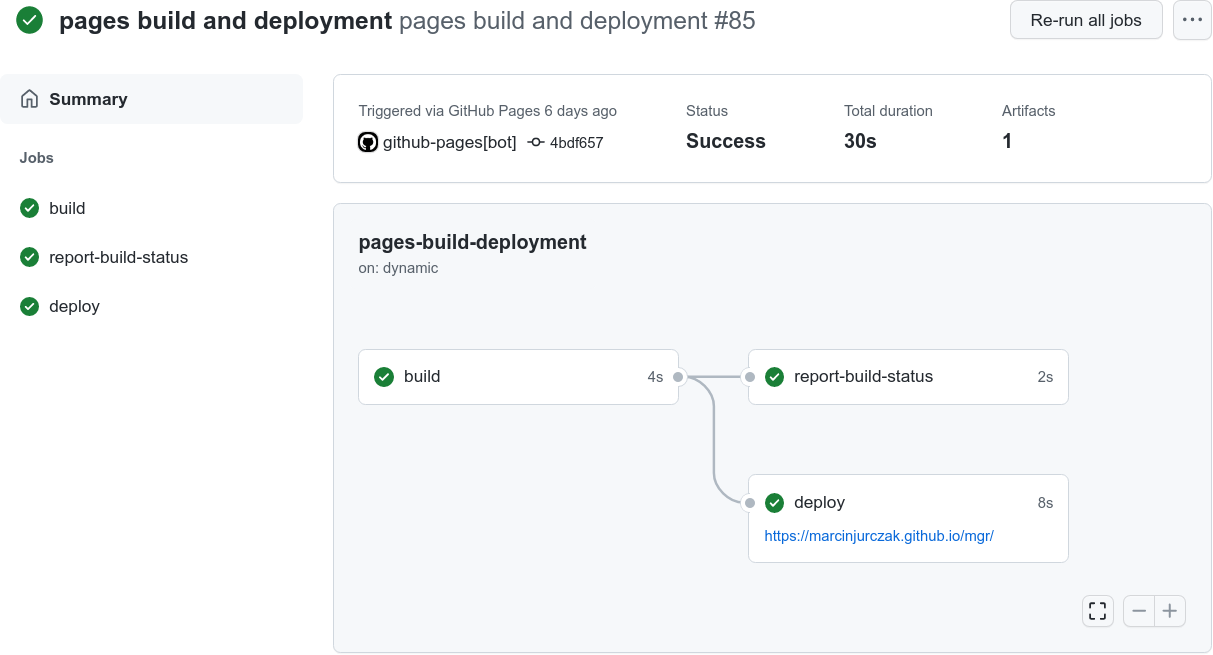
\includegraphics[width=0.95\textwidth]{img/deploy_yml.png}
    \caption{Publikacja aplikacji z użyciem GitHub Pages}\label{fig:deploy_yml}
\end{figure}

% ---------------------------------------------------------------------------------------------------------------------

\chapter{Podsumowanie}
Niniejszy rozdział ma na celu wskazanie efektów końcowych pracy magisterskiej i przedstawienie wyciągniętych wniosków na temat tworzenia aplikacji frontendowych wykorzystując język programowania Elm.

\section{Efekty}
W ramach pracy magisterskiej powstały dwie implementacje tej samej aplikacji internetowej typu \textit{startpage}, czyli strony startowej przeglądarki.
Pierwsza, główna implementacja została stworzona z wykorzystaniem języka funkcyjnego Elm, a druga w celach porównawczych przy pomocy biblioteki React.
Ponadto wdrożona została automatyzacja procesów ciągłej integracji i ciągłego dostarczania z wykorzystaniem zdalnego repozytorium kodu źródłowego GitHub i usług dostarczanych przez ten serwis, tj.~GitHub Actions oraz GitHub Pages.

Kolejnym efektem pracy magisterskiej jest niniejszy dokument, zawierający przede wszystkim opis implementacji stworzonej aplikacji, porównanie Elma z innymi rozwiązaniami tego typu pod kątem wydajnościowym jak i uwzględniając subiektywne odczucia towarzyszące podczas pracy z językiem.
Przygotowana została także instrukcja laboratoryjna przeprowadzająca czytelnika przez proces tworzenia oprogramowania z użyciem języka Elm, od przygotowania środowiska, przez podstawy języka, aż po stworzenie pełnej aplikacji frontendowej, wraz z ćwiczeniami.

\section{Wnioski}
Elm jest zdecydowanie bardzo ciekawym rozwiązaniem do tworzenia aplikacji frontedowych.
Zawiera świetną dokumentację i zestaw najpotrzebniejszych narzędzi, które umożliwiają szybkie i przyjemne tworzenie oprogramowania.

Stanowczo sprawdzi się w środowiskach produkcyjnych ze względu na swój brak występowania wyjątków w czasie działania programu, a także na możliwość automatyzacji procesów CI/CD, co udało mi się pokazać w poprzednim rozdziale.
Kod źródłowy wymaga trzymania sie ustalonej architektury, jednak w przypadku Elma przychodzi to dość naturalnie i powoduje, że kod jest bardzo czytelny i łatwy do zrozumienia.

% ---------------------------------------------------------------------------------------------------------------------

\listoffigures
% \listoftables
\lstlistoflistings{}

\printbibliography{}

% ---------------------------------------------------------------------------------------------------------------------

\end{document}

